\documentclass[10pt]{beamer}
\usefonttheme{professionalfonts}
%\usetheme{CambridgeUS}
%
% Choose how your presentation looks.
%
% For more themes, color themes and font themes, see:
% http://deic.uab.es/~iblanes/beamer_gallery/index_by_theme.html
%
\mode<presentation>
{
  \usetheme{default}      % or try Darmstadt, Madrid, Warsaw, ...
  \usecolortheme{beaver} % or try albatross, beaver, crane, ...
  \usefonttheme{default}  % or try serif, structurebold, ...
  \setbeamertemplate{navigation symbols}{}
  \setbeamertemplate{caption}[numbered]
} 

\usepackage[english]{babel}
\usepackage[utf8x]{inputenc}
\usepackage{tikz}
\usepackage{pgfplots}
\usepackage{array}  % for table column M
\usepackage{makecell} % to break line within a cell
\usepackage{verbatim}
\usepackage{graphicx}
\usepackage{epstopdf}
\usepackage{amsfonts}
\usepackage{xcolor}
\usepackage{ifthen}
%\usepackage{mathtools}
\usepackage[makeroom]{cancel}
\usetikzlibrary{spy}
%\captionsetup{compatibility=false}
%\usepackage{dsfont}
\usepackage[absolute,overlay]{textpos}
\usetikzlibrary{calc, angles,quotes}
\usetikzlibrary{pgfplots.fillbetween, backgrounds}
\usetikzlibrary{positioning}
\usetikzlibrary{arrows}
\usetikzlibrary{pgfplots.groupplots}
\usetikzlibrary{arrows.meta}
\usetikzlibrary{plotmarks}
\usetikzlibrary{decorations.markings}
\usepgfplotslibrary{groupplots}
\pgfplotsset{compat=newest} 
%\pgfplotsset{plot coordinates/math parser=false}

\usepackage{hyperref}
\hypersetup{
    colorlinks=true,
    linkcolor=blue,
    filecolor=magenta,      
    urlcolor=cyan,
}

%
%%% Page numbering
\usepackage{etoolbox} % necessary for excluding beamer-only frames from page numbering

\makeatletter
\pretocmd{\beamer@@@@frame}{\alt<#1>{}{\beamer@noframenumberingtrue}}{}{}
\makeatother

\addtobeamertemplate{navigation symbols}{}{%
	\usebeamerfont{footline}%
	\usebeamercolor[fg]{footline}%
	\hspace{1em}%
	\insertframenumber/\inserttotalframenumber
}
%%%

\definecolor{matlabcomment}{RGB}{34,139,34}

\pgfmathdeclarefunction{gauss}{1}{%
	\pgfmathparse{1/(sqrt(2*pi))*exp(-((#1)^2)/2)}%
}

\pgfmathdeclarefunction{laplacian}{2}{%
	\pgfmathparse{1/(#2*2)*exp(-(abs(x-#1))/(#2))}%
}

\pgfmathdeclarefunction{pretty_func}{1}{%
	\pgfmathparse{cos(deg(#1/2)) - sin(deg(#1)) + cos(deg(#1/2)-45) - sin(deg(#1/4)-154)}%
}

\pgfplotsset{
	dirac/.style={
		mark=triangle*,
		mark options={scale=2},
		ycomb,
		scatter,
		visualization depends on={y/abs(y)-1 \as \sign},
		scatter/@pre marker code/.code={\scope[rotate=90*\sign,yshift=-2pt]}
	}
}

\def\thickness{very thick}

\tikzset{
amark/.style 2 args={
	decoration={             
		markings, 
		mark=at position {0.5} with { 
			\arrow{stealth},
			\node[#2] {#1};
		}
	}, \thickness,
	postaction={decorate}
},
earlymark/.style 2 args={
	decoration={             
		markings, 
		mark=at position {0.25} with { 
			\arrow{stealth},
			\node[#2] {#1};
		}
	}, \thickness,
	postaction={decorate}
},
latemark/.style 2 args={
	decoration={             
		markings, 
		mark=at position {0.8} with { 
			\arrow{stealth},
			\node[#2] {#1};
		}
	}, \thickness,
	postaction={decorate}
},
zpath/.style={
	decoration={             
		markings, 
		mark=at position {0.5} with { 
			\arrow{stealth},
			\node[#1] {$z^{-1}$};
		}
	}, \thickness,
	postaction={decorate}
},
terminal/.style 2 args={draw,circle,inner sep=2pt,label={#1:#2}},
}


\tikzset{
	invisible/.style={opacity=0},
	visible on/.style={alt={#1{}{invisible}}},
	alt/.code args={<#1>#2#3}{%
		\alt<#1>{\pgfkeysalso{#2}}{\pgfkeysalso{#3}} % \pgfkeysalso doesn't change the path
	},
}

\newcommand\PlotSampledSpectrum[4]{%
	\def\fs{#2}%
	\def\fmax{#3}%
	\def\ros{#4}%
	\input{#1}%
}

\pgfmathdeclarefunction{invgauss}{2}{%
	\pgfmathparse{sqrt(-2*ln(#1))*cos(deg(2*pi*#2))}%
}

\tikzset{
	declare function={
		sinc(\x) = (and(\x!=0, 1) * (sin(deg(pi*\x))/(pi*\x)) +
		(and(\x==0, 1) * 1);
	}
}

\DeclareMathOperator{\E}{\mathbb{E}} % expectation

\newcolumntype{M}[1]{>{\centering\arraybackslash}m{#1}}

\definecolor{blue2}{RGB}{51, 105, 232}  
\definecolor{red2}{RGB}{213, 15, 37}  
\definecolor{green2}{RGB}{0, 153, 37}  
\definecolor{green3}{rgb}{0.1922, 0.6392, 0.3294}% 
\definecolor{yellow2}{RGB}{238, 178, 17} 
\definecolor{gray2}{RGB}{102, 102, 102}
\definecolor{orange2}{RGB}{230, 85, 13}

% Qualitative pallete set1 from www.ColorBrewer.org
\definecolor{Qred}{RGB}{228,26,28}
\definecolor{Qblue}{RGB}{55,126,184}
\definecolor{Qgreen}{RGB}{77,175,74}
\definecolor{Qpurple}{RGB}{152,78,163}
\definecolor{Qorange}{RGB}{255,127,0}
\definecolor{Qyellow}{RGB}{255,255,51}
\definecolor{Qbrown}{RGB}{166,86,40}
\definecolor{Qpink}{RGB}{247,129,191}
\definecolor{Qgray}{RGB}{153,153,153}

\newcommand\SimpleSys[4]{%
	\def\xin{#2}%
	\def\Hz{#3}%
	\def\yout{#4}
	\input{#1}%
} % some definitions

%% 
\title[EE 264]{Filter Design}
\author{Jose Krause Perin}
\institute{Stanford University}
\date{August 3, 2017}

\begin{document}

\begin{frame}
  \titlepage
\end{frame}

%
%\begin{frame}{Announcements}
%	\begin{itemize}
%		\item Homework \#4 due on Sunday, July 30. Start early!
%		\item Midterm review session will be on Friday at 1:30pm at \textbf{Gates B03}
%		\item Please fill out the mid-quarter teaching evaluation survey and get 2\% extra credit: \url{https://tinyurl.com/y8cyfddy}. \textbf{Deadline:} Today
%		\item We'll release practice midterms today. Their solutions will be released on Friday after the review session.
%	\end{itemize}
%\end{frame}

%
\begin{frame}{Last lecture}
\begin{itemize}
	\item Two's complement is a fixed-point representation that allows fractions to be represented as integers
	\item There's an inherent trade-off between roundoff noise and overflow/clipping
	\item FIR systems remain stable after coefficient quantization
	\item Linear phase FIR systems remain linear phase after coefficient quantization, since the impulse response remains symmetric
	\item Coefficient quantization may lead to instability in IIR systems, as poles may move outside the unit circle
	\item Similarly to quantization noise, roundoff noise is modeled by an additive white noise that is independent of the input signal (the linear noise model).
	\item Roundoff noise is minimized by performing quantization only after accumulation, but this requires $(2B+1)$-bit adders
	\item In FIR structures the equivalent roundoff noise at the output is white
	\item IIR structures lead to roundoff noise shaping
	\item Least noisy IIR structure depends on the system
	\item Cascade and parallel forms are used to mitigate total roundoff noise
\end{itemize}
\end{frame}

%
\section{Outline}

\begin{frame}{Practice and theory}
\begin{block}{In practice}
	\vspace{-0.5cm}
	\begin{center}
		\resizebox{\linewidth}{!}{\def\layersep{1.5cm}
\def\outsep{0.7cm}
\def\dy{1.25}

\begin{tikzpicture}[->, >=stealth, shorten >= 0pt, draw=black!50, node distance=\layersep, font=\sffamily]
    \tikzstyle{node}=[circle,fill=black,minimum size=2pt,inner sep=0pt]
    \tikzstyle{block}=[draw=black,rectangle,fill=none,minimum size=1.5cm, inner sep=0pt]
    \tikzstyle{annot} = []

	\node[node] (xc) at (0, -\dy cm) {};
    \node[block] (ADC) at (1*\layersep, -\dy cm) {ADC};
    \node[block, text width = 2.5cm, align= center] (DSP) at (3*\layersep, -\dy cm) {Digital Signal Processor};
    \node[block] (DAC) at (5*\layersep, -\dy cm) {DAC};
	\coordinate (yc) at (6*\layersep, -\dy cm) {};
	
	\coordinate (mid1) at ($(ADC.east)!0.5!(DSP.west)$) {};
	\coordinate (mid2) at ($(DSP.east)!0.5!(DAC.west)$) {};
		
    \path (xc) edge (ADC);
    \path (ADC) edge (DSP);
    \path (DSP) edge (DAC);
    \path (DAC) edge (yc);
    
    \node[above = 0.5mm of mid1] {$x[n]$};
    \node[above = 0.5mm of mid2] {$y[n]$};
    \node[left = 0mm of xc, text width = 1cm, align=center] {$x_c(t)$};
    \node[right = 0mm of yc, text width = 1cm, align=center] {$y_c(t)$}; 
    

\end{tikzpicture}}
	\end{center}
\end{block}

\begin{block}{DSP theory}
	\vspace{-0.5cm}
	\begin{center}
		\def\Heff{1}
		\resizebox{\linewidth}{!}{\def\layersep{2cm}
\def\outsep{0.7cm}
\def\dy{1.25}

\begin{tikzpicture}[->, >=stealth, shorten >= 0pt, draw=black!50, node distance=\layersep, font=\sffamily]
    \tikzstyle{node}=[circle,fill=black,minimum size=2pt,inner sep=0pt]
    \tikzstyle{block}=[draw=black,rectangle,fill=none,minimum size=1.5cm, inner sep=0pt]
    \tikzstyle{annot} = []

	\node[node] (xc) at (0, -\dy cm) {};
    \node[block] (ADC) at (1*\layersep, -\dy cm) {C-to-D};
    \node[block, text width = 2cm, align= center] (DSP) at (3*\layersep, -\dy cm) {LTI \\ System};
    \node[block] (DAC) at (5*\layersep, -\dy cm) {D-to-C};
	\coordinate (yc) at (6*\layersep, -\dy cm) {};
	
	\coordinate (mid1) at ($(ADC.east)!0.5!(DSP.west)$) {};
	\coordinate (mid2) at ($(DSP.east)!0.5!(DAC.west)$) {};
		
    \path (xc) edge (ADC);
    \path (ADC) edge (DSP);
    \path (DSP) edge (DAC);
    \path (DAC) edge (yc);
    
    \node[above = 0.5mm of mid1] {$x[n]$};
    \node[below = 0.5mm of mid1] {$X(e^{j\omega})$};
    \node[above = 0.5mm of mid2] {$y[n]$};
    \node[below = 0.5mm of mid2] {$Y(e^{j\omega})$};
    \node[above = 0mm of xc, text width = 1cm, align=center] {$x_c(t)$};
    \node[below = 0mm of xc, text width = 1cm, align=center] {$X_c(j\Omega)$};
    \node[above = 0mm of yc, text width = 1cm, align=center] {$y_r(t)$}; 
    \node[below = 0mm of yc, text width = 1cm, align=center] {$Y_r(j\Omega)$};
    \node at ($(DSP.south)-(0, 0.25cm)$) {$h[n] \leftrightarrow H(e^{j\omega})$};
\end{tikzpicture}}
	\end{center}
\end{block}

\end{frame}

\begin{frame}{Digital filter design}
	We'll cover two different design problems
	\begin{enumerate}
		\item Digital filter design \underline{from analog filter}
		
		Given a continuous-time LTI filter defined by $h_{eq}(t) \Longleftrightarrow H_{eq}(s)$, how to obtain the corresponding discrete-time filter $h[n] \Longleftrightarrow H(z)$ such that
		\begin{equation*}
			H(e^{j\Omega T}) \approx H_{eq}(j\Omega), |\Omega| < \Omega_s/2
		\end{equation*}
		
		\textbf{Design techniques:}
		\begin{itemize}
			\item Impulse invariance
			\item Bilinear transformation
		\end{itemize}
		Design by impulse invariance can result in either FIR or IIR filters, whereas bilinear transformation generally results in IIR filters. 
	\end{enumerate}
\end{frame}

%
\begin{frame}{Digital filter design}
\begin{enumerate}\setcounter{enumi}{1}
	\item Digital FIR filter design \underline{from specifications}
	
	How to find FIR $H(z)$ such that $H(e^{j\omega})$ best approximates a desired frequency response $H_d(e^{j\omega})$? Essentially a polynomial curve fitting problem.
	\begin{center}
		\resizebox{0.6\linewidth}{!}{\begin{tikzpicture}
\begin{axis}[
name=plot1,
axis lines*=middle,
enlargelimits = upper, clip=false,
scale only axis,
axis on top=false,
axis line style={->,>=stealth},
width=0.6\textwidth,
height=0.4\textwidth,
xlabel={$\omega$},
ylabel={$H_d(e^{j\omega})$},
every axis x label/.style={
	at={(ticklabel* cs:1)},
	xshift=-0.2cm,
	anchor=north,
},
every axis y label/.style={
	at={(ticklabel* cs:1)},
	xshift=0.4cm,
	%yshift=0.35cm,
	anchor=south,
},
every outer x axis line/.append style={white!15!black},
every x tick label/.append style={font=\color{white!15!black}},
xmin=0, xmax=1,
ymin=0, ymax=1.25,
ytick={0.2, 0.9, 1.1}, yticklabels={$\delta_2$, $1-\delta_1$, $1+\delta_1$},
xtick={0, 0.25, 0.6, 1},
xticklabels ={$0$, $\omega_p$, $\omega_s$, $\pi$},
every outer y axis line/.append style={white!15!black},
every y tick label/.append style={font=\color{white!15!black}},
legend style={draw=white!15!black,fill=white,legend cell align=left}]
\addplot[solid, line width=1pt, domain=0:0.25, samples=2] {1.1}; 
\addplot[solid, line width=1pt, domain=0:0.25, samples=2] {0.9};
\addplot[solid, line width=1pt, domain=0.6:1, samples=2] {0.2};

\addplot[blue2, line width=2pt, domain=0:0.25, samples=2] {1};
\addplot[blue2, line width=2pt, domain=0.6:1, samples=2] {0};
\addplot[dashed, line width=1pt] coordinates {(0.25, 0) (0.25, 0.9)};
\addplot[dashed, line width=1pt] coordinates {(0.6, 0) (0.6, 0.9)};

\fill [black!20] (axis cs: 0, 1.1) rectangle (0.25, 1.2);
\fill [black!20] (axis cs: 0, 0.9) rectangle (0.25, 0.8);
\fill [black!20] (axis cs: 0.6, 0.2) rectangle (1, 0.3);

\node[align=center, text width = 2cm, scale=0.8] at ($(axis cs: 0, 0.5)!0.5!(axis cs: 0.25, 0.5)$) {Passband};
\node[align=center, text width = 2cm, scale=0.8] at ($(axis cs: 0.6, 0.5)!0.5!(axis cs: 1, 0.5)$) {Stopband};

\ifdefined\CARE
	\fill [red!30] (axis cs: 0.25, 0) rectangle (axis cs: 0.6, 1);
	\node[align=center, text width = 2cm, scale=0.8] at ($(axis cs: 0.25, 0.5)!0.5!(axis cs: 0.6, 0.5)$) {Don't care};
\else
	\node[align=center, text width = 2cm, scale=0.8] at ($(axis cs: 0.25, 0.5)!0.5!(axis cs: 0.6, 0.5)$) {Transition};
\fi

\end{axis}

\ifdefined\CARE
	\node[blue2, below=0.5cm, align=right, text width = 2.5cm, scale=0.8] (t1) at ($(plot1.south west)$) {$W(\omega \leq \omega_p) = 1$};
	\node[red2, below=0.5cm, right=0.01cm of t1, align=center, text width = 4cm, scale=0.8] (t2) {$W(\omega_p < \omega < \omega_s) = 0$};
	\node[blue2, below=0.5cm, right=0.01cm of t2, align=center, text width = 2.5cm, scale=0.8] (t3) {$W(\omega \geq \omega_s) = 1$};
\fi
\end{tikzpicture}}
	\end{center}
	
	\textbf{Design techniques:}
	\begin{itemize}
		\item Window method
		\item Optimal filter design
		\begin{itemize}
			\item Parks-McClellan algorithm
			\item Least-squares algorithm
		\end{itemize}
	\end{itemize}
\end{enumerate}
\end{frame}

%
\begin{frame}{Outline}
	\tableofcontents
\end{frame}

\section{Design from Analog Filter}
\begin{frame}{Digital processing of analog signals}
\begin{center}
	\def\Heff{1}
	\resizebox{\linewidth}{!}{\def\layersep{2cm}
\def\outsep{0.7cm}
\def\dy{1.25}

\begin{tikzpicture}[->, >=stealth, shorten >= 0pt, draw=black!50, node distance=\layersep, font=\sffamily]
    \tikzstyle{node}=[circle,fill=black,minimum size=2pt,inner sep=0pt]
    \tikzstyle{block}=[draw=black,rectangle,fill=none,minimum size=1.5cm, inner sep=0pt]
    \tikzstyle{annot} = []

	\node[node] (xc) at (0, -\dy cm) {};
    \node[block] (ADC) at (1*\layersep, -\dy cm) {C-to-D};
    \node[block, text width = 2cm, align= center] (DSP) at (3*\layersep, -\dy cm) {LTI \\ System};
    \node[block] (DAC) at (5*\layersep, -\dy cm) {D-to-C};
	\coordinate (yc) at (6*\layersep, -\dy cm) {};
	
	\coordinate (mid1) at ($(ADC.east)!0.5!(DSP.west)$) {};
	\coordinate (mid2) at ($(DSP.east)!0.5!(DAC.west)$) {};
		
    \path (xc) edge (ADC);
    \path (ADC) edge (DSP);
    \path (DSP) edge (DAC);
    \path (DAC) edge (yc);
    
    \node[above = 0.5mm of mid1] {$x[n]$};
    \node[below = 0.5mm of mid1] {$X(e^{j\omega})$};
    \node[above = 0.5mm of mid2] {$y[n]$};
    \node[below = 0.5mm of mid2] {$Y(e^{j\omega})$};
    \node[above = 0mm of xc, text width = 1cm, align=center] {$x_c(t)$};
    \node[below = 0mm of xc, text width = 1cm, align=center] {$X_c(j\Omega)$};
    \node[above = 0mm of yc, text width = 1cm, align=center] {$y_r(t)$}; 
    \node[below = 0mm of yc, text width = 1cm, align=center] {$Y_r(j\Omega)$};
    \node at ($(DSP.south)-(0, 0.25cm)$) {$h[n] \leftrightarrow H(e^{j\omega})$};
\end{tikzpicture}}
\end{center}

As long as there is no aliasing and that the reconstruction filter is the ideal lowpass filter these equalities hold:

\begin{equation}
H_{eq}(j\Omega) = \begin{cases}
H(e^{j\Omega T}), & |\Omega| < \pi/T \\
0, & |\Omega| > \pi/T
\end{cases} \tag{from DSP to analog}
\end{equation}

\begin{equation}
H(e^{j\omega}) = H_{eq}(j\omega/T), \quad|\omega| < \pi  \tag{from analog to DSP}
\end{equation}

In practice, these are good approximations.
\end{frame}

\subsection{Impulse Invariance}
\begin{frame}{Impulse invariance}

\textbf{Question:} How to design $h[n] \longleftrightarrow H(z)$ if we know $h_{eq}(t) \longleftrightarrow H_{eq}(s)$?

\begin{center}
	\def\Heff{1}
	\resizebox{\linewidth}{!}{\def\layersep{2cm}
\def\outsep{0.7cm}
\def\dy{1.25}

\begin{tikzpicture}[->, >=stealth, shorten >= 0pt, draw=black!50, node distance=\layersep, font=\sffamily]
    \tikzstyle{node}=[circle,fill=black,minimum size=2pt,inner sep=0pt]
    \tikzstyle{block}=[draw=black,rectangle,fill=none,minimum size=1.5cm, inner sep=0pt]
    \tikzstyle{annot} = []

	\node[node] (xc) at (0, -\dy cm) {};
    \node[block] (ADC) at (1*\layersep, -\dy cm) {C-to-D};
    \node[block, text width = 2cm, align= center] (DSP) at (3*\layersep, -\dy cm) {LTI \\ System};
    \node[block] (DAC) at (5*\layersep, -\dy cm) {D-to-C};
	\coordinate (yc) at (6*\layersep, -\dy cm) {};
	
	\coordinate (mid1) at ($(ADC.east)!0.5!(DSP.west)$) {};
	\coordinate (mid2) at ($(DSP.east)!0.5!(DAC.west)$) {};
		
    \path (xc) edge (ADC);
    \path (ADC) edge (DSP);
    \path (DSP) edge (DAC);
    \path (DAC) edge (yc);
    
    \node[above = 0.5mm of mid1] {$x[n]$};
    \node[below = 0.5mm of mid1] {$X(e^{j\omega})$};
    \node[above = 0.5mm of mid2] {$y[n]$};
    \node[below = 0.5mm of mid2] {$Y(e^{j\omega})$};
    \node[above = 0mm of xc, text width = 1cm, align=center] {$x_c(t)$};
    \node[below = 0mm of xc, text width = 1cm, align=center] {$X_c(j\Omega)$};
    \node[above = 0mm of yc, text width = 1cm, align=center] {$y_r(t)$}; 
    \node[below = 0mm of yc, text width = 1cm, align=center] {$Y_r(j\Omega)$};
    \node at ($(DSP.south)-(0, 0.25cm)$) {$h[n] \leftrightarrow H(e^{j\omega})$};
\end{tikzpicture}}
\end{center}

Design $h[n]$ by sampling $h_{eq}(t)$ with period $T$.
\begin{equation}
	h[n] = Th_c(nT) \tag{impulse invariance}
\end{equation}

The scaling factor $T$ compensates for the $1/T$ attenuation in the frequency domain due to sampling

The resulting $h[n]$ depends on the sampling period $T$.

\end{frame}

\begin{frame}{Impulse invariance example: lowpass Butterworth filter}
Butterworth filters are \textbf{maximally flat} in the passband and are monotonic overall. The downside of Butterworth filter is their relatively slow roll-off.
\vspace{0.25cm}

For this example, consider the following 6th-order continuous-time lowpass Butterworth filter:

\begin{align*}
&H_{eq}(s)  \\
&= \frac{0.12093}{(s^2 + 0.364s + 0.4945)(s^2 + 0.9945s + 0.4945)(s^2 + 1.3385 + 0.4945)}
\end{align*}

\end{frame}

%
\begin{frame}{Impulse invariance example: lowpass Butterworth filter}
To design an \textbf{FIR filter} by impulse invariance we must
\begin{enumerate}
	\item Obtain the continuous-time impulse response $h_{eq}(t) \longleftrightarrow H_{eq}(s)$ (\texttt{impulse} in Matlab)
	\item Sample and scale $h_{eq}(t)$ with period $T$ and record only $M+1$ first samples 
	\begin{equation*}
		h[n] = \begin{cases}
		Th_{eq}(nT), & n = 0, \ldots, M \\
		0, & \text{otherwise}
		\end{cases}, \tag{for causal $h_{eq}(t)$}
	\end{equation*}
	$h[n]$ is the FIR filter coefficients. $M$ is typically chosen to satisfy some energy criterion. For instance, samples must contain $95\%$ of the signal energy.
\end{enumerate} 
\begin{center}
	\resizebox{0.7\linewidth}{!}{\begin{tikzpicture}
\begin{axis}[
	name=plot1,
	axis lines*=middle,
	enlargelimits = false, clip=true,
	scale only axis,
	width=0.7\textwidth,
	height=0.3\textwidth,
	ymin=-0.1,	ymax=0.28,
	xmin=0, xmax=24.5,
	axis line style={->,>=stealth, shorten >= -0.5cm},
	xlabel={\small $t$},
	ylabel={\small $h_{eq}(t)$},
	every axis x label/.style={
		at={(ticklabel* cs:1)},
		xshift=0.5cm,
		anchor=north,
	},
	every axis y label/.style={
		at={(ticklabel* cs:1)},
		anchor=south,
		xshift=0.5cm,
	},
	xtick={0, 1, 5, 24},
	xticklabels={0, $T$, $5T$, $24T$},
	ytick=\empty,
	every outer y axis line/.append style={white!15!black},
	every y tick label/.append style={font=\color{white!15!black}},
	legend style={draw=white!15!black,fill=white,legend cell align=left}]
	
	\addplot [smooth, color=black, solid, line width=1.5pt] table[x index=0,y index=1] {figs/data/imp_invar_samples.dat};
	
	\only<2|handout:1>{
	\addplot [ycomb, color=red2, mark=*, fill=white, mark options={scale=1, fill=white}, line width=1.5pt, each nth point={4}] table[x index=0,y index=1] {figs/data/imp_invar_samples.dat};
}
\end{axis}
\end{tikzpicture}}
\end{center}

\end{frame}

%
\begin{frame}{Impulse invariance example: lowpass Butterworth filter}

\begin{columns}
	\begin{column}{0.5\textwidth}
		\textbf{Magnitude}
		\begin{center}
			\resizebox{\linewidth}{!}{\begin{tikzpicture}
\begin{axis}[
name=plot2a,
%at=(plot2.below south east), anchor=above north east,
xshift=1cm,
axis lines*=middle,
enlargelimits = upper, clip=true,
scale only axis,
axis line style={->,>=stealth},
xlabel={$\omega$},
ylabel={dB},
every axis x label/.style={
	at={(ticklabel* cs:1)},
	xshift=-0.2cm,
	anchor=north,
},
every axis y label/.style={
	at={(ticklabel* cs:1)},
	xshift=0.4cm,
	%yshift=0.35cm,
	anchor=south,
},
every outer x axis line/.append style={white!15!black},
every x tick label/.append style={font=\color{white!15!black}},
xmin=0, xmax=1,
ymin=-60, ymax=0,
xtick={0, 0.25, 0.5, 0.75, 1},
xticklabels ={$0$, $\pi/4$, $\pi/2$, $3\pi/4$, $\pi$},
ymajorgrids,
every outer y axis line/.append style={white!15!black},
every y tick label/.append style={font=\color{white!15!black}},
legend style={draw=white!15!black,fill=white,legend cell align=left, at={(axis cs: 1.05, -5)}}]

\addplot [smooth, color=black, solid, line width=2pt] table[x index=0,y index=1] {figs/data/imp_invar_FIR_butter_fir_mag_Hc.dat}; \addlegendentry{$H_{eq}(j\Omega)$};

\addplot [smooth, color=red2, solid, line width=2pt]
table[x index=0,y index=1] {figs/data/imp_invar_FIR_butter_fir_mag_Hfir.dat}; \addlegendentry{$H(e^{j\omega})$ FIR 25 samples};

\only<2-|handout:0> {
\addplot [smooth, color=blue2, solid, line width=2pt]
table[x index=0,y index=1] {figs/data/imp_invar_FIR_butter_fir_mag10_Hfir.dat}; \addlegendentry{$H(e^{j\omega})$ FIR 10 samples};
}

\only<3-|handout:0> {
	
	\addplot [smooth, color=black, solid, line width=2pt, forget plot] table[x index=0,y index=1] {figs/data/imp_invar_FIR_butter_fir_mag_T2_Hc.dat};
	
	\addplot [smooth, color=green2, solid, line width=2pt]
	table[x index=0,y index=1] {figs/data/imp_invar_FIR_butter_fir_mag_T2_Hfir.dat}; \addlegendentry{$H(e^{j\omega})$ $T_2 = 0.5T$};
}

\end{axis}
\end{tikzpicture}}
		\end{center}
	\end{column}
	\begin{column}{0.5\textwidth}
		\textbf{Phase}
		\begin{center}
			\resizebox{\linewidth}{!}{\begin{tikzpicture}
\begin{axis}[
name=plot2a,
%at=(plot2.below south east), anchor=above north east,
xshift=1cm,
axis lines*=middle,
enlargelimits = upper, clip=true,
scale only axis,
axis line style={->,>=stealth},
xlabel={$\omega$},
ylabel={rad},
every axis x label/.style={
	at={(ticklabel* cs:1)},
	xshift=-0.2cm,
	anchor=north,
},
every axis y label/.style={
	at={(ticklabel* cs:1)},
	xshift=0.4cm,
	%yshift=0.35cm,
	anchor=south,
},
every outer x axis line/.append style={white!15!black},
every x tick label/.append style={font=\color{white!15!black}},
xmin=0, xmax=1,
ymin=-10, ymax=0,
xtick={0, 0.25, 0.5, 0.75, 1},
xticklabels ={$0$, $\pi/4$, $\pi/2$, $3\pi/4$, $\pi$},
ymajorgrids,
every outer y axis line/.append style={white!15!black},
every y tick label/.append style={font=\color{white!15!black}},
legend style={draw=white!15!black,fill=white,legend cell align=left, at={(axis cs: 1.05, -2)}}]

\addplot [smooth, color=black, solid, line width=2pt] table[x index=0,y index=1] {figs/data/imp_invar_FIR_butter_fir_phase_Hc.dat}; \addlegendentry{$H_{eq}(j\Omega)$};

\addplot [smooth, color=red2, solid, line width=2pt]
table[x index=0,y index=1] {figs/data/imp_invar_FIR_butter_fir_phase_Hfir.dat}; \addlegendentry{$H(e^{j\omega})$ FIR 25 samples};

\only<2-|handout:0> {
	\addplot [smooth, color=blue2, solid, line width=2pt]
	table[x index=0,y index=1] {figs/data/imp_invar_FIR_butter_fir_phase10_Hfir.dat}; \addlegendentry{$H(e^{j\omega})$ FIR 10 samples};
}

\only<3-|handout:0> {
	
	\addplot [smooth, color=black, solid, line width=2pt, forget plot] table[x index=0,y index=1] {figs/data/imp_invar_FIR_butter_fir_phase_T2_Hc.dat};
	
	\addplot [smooth, color=green2, solid, line width=2pt]
	table[x index=0,y index=1] {figs/data/imp_invar_FIR_butter_fir_phase_T2_Hfir.dat}; \addlegendentry{$H(e^{j\omega})$ $T_2 = 0.5T$};
}

\end{axis}
\end{tikzpicture}}
		\end{center}
	\end{column}
\end{columns}

\vspace{0.2cm}
\textbf{Questions:}
\begin{enumerate}
	\item What would happen if we take fewer samples (smaller $M$)?
	\item What would happen if we decrease the sampling period e.g., $T_2 = 0.5T$?
\end{enumerate}

\end{frame}

%
\begin{frame}{Impulse invariance example: lowpass Butterworth filter}

\begin{itemize}
	\item Designing FIR filters by impulse invariance is straightforward. Plus, FIR systems have the implementation advantages discussed in lectures 7 and 8
	\item \textbf{Problem:} it may require prohibitively many samples to achieve good accuracy
	\item IIR systems generally offer better accuracy while requiring fewer operations (coefficients)
\end{itemize}

To design an \textbf{IIR filter} by impulse invariance we must

\begin{enumerate}
	\item Invert the Laplace transform $H_{eq}(s)$ using \textbf{partial fraction expansion} to obtain $h_{eq}(t)$ analytically. Function \texttt{residue} in Matlab	
	\item Sample $h_{eq}(t)$: $h[n] = Th_{eq}(nT)$
	\item Calculate the $z$-transform $H(z)$ of $h[n]$
\end{enumerate}
\end{frame}


%
\begin{frame}{Impulse invariance example: lowpass Butterworth filter}

For the 6th-order Butterworth example:

\begin{columns}
	\begin{column}{0.5\textwidth}
		\begin{align*}
		H(z) =& \frac{0.2871 -0.4466z^{-1}}{1 -1.2971z^{-1} + 0.6949z^{-2}} \\ &+\frac{-2.1428 +1.1455z^{-1}}{1 -1.0691z^{-1} + 0.3699z^{-2}}  \\
		&+\frac{1.8557 - 0.6303z^{-1}}{1 -0.9972^{-1} + 0.2570z^{-2}} 
		\end{align*}
	\end{column}
	
	\begin{column}{0.5\textwidth}
		\begin{center}
			\resizebox{\linewidth}{!}{\begin{tikzpicture}
\begin{axis}[
axis equal,
axis lines*=middle,
enlargelimits = false, clip=true,
xmin=-1.40,
xmax=1.39,
ymin=-1.10,
ymax=1.10,
axis line style={->,>=stealth},
xlabel={$\mathrm{Re}\{z\}$},
ylabel={$\mathrm{Im}\{z\}$},
every axis x label/.style={
at={(ticklabel* cs:1)},
anchor=north,
},
every axis y label/.style={
at={(ticklabel* cs:1)},
anchor=south,
},
xmajorgrids,
ymajorgrids,
every outer y axis line/.append style={white!15!black},
every y tick label/.append style={font=\color{white!15!black}},
legend style={draw=white!15!black,fill=white,legend cell align=left}]
\draw (axis cs:0,0) circle [black!50, dashed, line width=2pt, radius=1];
\addplot [line width=1pt,mark=x, only marks, mark size = 3pt]
table[row sep=crcr]{
	0.64855 0.52372 \\
	0.64855 -0.52372 \\
	0.53455 0.2901 \\
	0.53455 -0.2901 \\
	0.4986 0.091641 \\
	0.4986 -0.091641 \\
};

\addplot [line width=1pt,mark=*, only marks, mark size = 3pt, mark options={fill=white}]
table[row sep=crcr]{
	0 0 \\
	-14.1544 0 \\
	-1.4649 0 \\
	-0.27662 0 \\
	-0.028546 0 \\
};

\end{axis}
\end{tikzpicture}}
		\end{center}
	\end{column}
\end{columns}
\end{frame}

%
\begin{frame}{Impulse invariance example: lowpass Butterworth filter}

\begin{columns}
	\begin{column}{0.5\textwidth}
		\textbf{Magnitude}
		\begin{center}
			\resizebox{\linewidth}{!}{\begin{tikzpicture}
\begin{axis}[
name=plot2a,
%at=(plot2.below south east), anchor=above north east,
xshift=1cm,
axis lines*=middle,
enlargelimits = upper, clip=true,
scale only axis,
axis line style={->,>=stealth},
xlabel={$\omega$},
ylabel={dB},
every axis x label/.style={
	at={(ticklabel* cs:1)},
	xshift=-0.2cm,
	anchor=north,
},
every axis y label/.style={
	at={(ticklabel* cs:1)},
	xshift=0.4cm,
	%yshift=0.35cm,
	anchor=south,
},
every outer x axis line/.append style={white!15!black},
every x tick label/.append style={font=\color{white!15!black}},
xmin=0, xmax=1,
ymin=-60, ymax=0,
xtick={0, 0.25, 0.5, 0.75, 1},
xticklabels ={$0$, $\pi/4$, $\pi/2$, $3\pi/4$, $\pi$},
ymajorgrids,
every outer y axis line/.append style={white!15!black},
every y tick label/.append style={font=\color{white!15!black}},
legend style={draw=white!15!black,fill=white,legend cell align=left, at={(axis cs: 1.05, -5)}}]

\addplot [smooth, color=black, solid, line width=2pt] table[x index=0,y index=1] {figs/data/imp_invar_FIR_butter_fir_mag_Hc.dat}; \addlegendentry{$H_{eq}(j\Omega)$};

\addplot [smooth, color=red2, solid, line width=2pt]
table[x index=0,y index=1] {figs/data/imp_invar_IIR_butter_mag_Hiir.dat}; \addlegendentry{$H(e^{j\omega})$ IIR};

\end{axis}
\end{tikzpicture}}
		\end{center}
	\end{column}
	\begin{column}{0.5\textwidth}
		\textbf{Phase}
		\begin{center}
			\resizebox{\linewidth}{!}{\begin{tikzpicture}
\begin{axis}[
name=plot2a,
%at=(plot2.below south east), anchor=above north east,
xshift=1cm,
axis lines*=middle,
enlargelimits = upper, clip=true,
scale only axis,
axis line style={->,>=stealth},
xlabel={$\omega$},
ylabel={rad},
every axis x label/.style={
	at={(ticklabel* cs:1)},
	xshift=-0.2cm,
	anchor=north,
},
every axis y label/.style={
	at={(ticklabel* cs:1)},
	xshift=0.4cm,
	%yshift=0.35cm,
	anchor=south,
},
every outer x axis line/.append style={white!15!black},
every x tick label/.append style={font=\color{white!15!black}},
xmin=0, xmax=1,
ymin=-10, ymax=0,
xtick={0, 0.25, 0.5, 0.75, 1},
xticklabels ={$0$, $\pi/4$, $\pi/2$, $3\pi/4$, $\pi$},
ymajorgrids,
every outer y axis line/.append style={white!15!black},
every y tick label/.append style={font=\color{white!15!black}},
legend style={draw=white!15!black,fill=white,legend cell align=left, at={(axis cs: 1.05, -2)}}]

\addplot [smooth, color=black, solid, line width=2pt] table[x index=0,y index=1] {figs/data/imp_invar_FIR_butter_fir_phase_Hc.dat}; \addlegendentry{$H_{eq}(j\Omega)$};

\addplot [smooth, color=red2, solid, line width=2pt]
table[x index=0,y index=1] {figs/data/imp_invar_IIR_butter_phase_Hiir.dat}; \addlegendentry{$H(e^{j\omega})$ IIR};

\end{axis}
\end{tikzpicture}}
		\end{center}
	\end{column}
\end{columns}

\begin{itemize}
	\item IIR systems achieve better accuracy while requiring fewer operations (coefficients) than FIR systems.
	\item Similarly to FIR systems, if we change the sampling frequency the behavior of the filter changes.
\end{itemize}
\end{frame}

%
\subsection{Bilinear Transformation}
\begin{frame}<beamer:1|handout:0>{Outline} 
\tableofcontents[currentsubsection]
\end{frame}

%
\begin{frame}{Bilinear transformation}
Another way to answer the question: How to design $h[n] \longleftrightarrow H(z)$ if we know $h_{eq}(t) \longleftrightarrow H_{eq}(s)$?
~\\
~\\

The \textbf{bilinear transformation} maps the left-hand side of the $s$-plane into the unit circle in the $z$-plane.
	
\begin{equation*}
	s = \frac{2}{T}\bigg(\frac{1 - z^{-1}}{1 + z^{-1}}\bigg) \tag{Bilinear transformation}
\end{equation*}

\begin{center}
	\resizebox{0.9\linewidth}{!}{\begin{tikzpicture}
\begin{axis}[
name=plot1,
axis equal,
axis lines*=middle,
enlargelimits = false, clip=true,
axis on top=true,
axis line style={->,>=stealth},
xlabel={$\sigma$},
ylabel={$\Omega$},
every axis x label/.style={
	at={(ticklabel* cs:1)},
	xshift=-0.2cm,
	anchor=north,
},
every axis y label/.style={
	at={(ticklabel* cs:1)},
	xshift=0.4cm,
	%yshift=0.35cm,
	anchor=south,
},
every outer x axis line/.append style={white!15!black},
every x tick label/.append style={font=\color{white!15!black}},
xmin=-2, xmax=2,
ymin=-2, ymax=2,
xtick=\empty,
ytick=\empty,
every outer y axis line/.append style={white!15!black},
every y tick label/.append style={font=\color{white!15!black}},
legend style={draw=white!15!black,fill=white,legend cell align=left}]

\fill[black!20] (axis cs:-3, -2) rectangle (0, 1.8);

\end{axis}

\begin{axis}[
name=plot2,
axis equal,
at=(plot1.east), anchor=west, xshift=1cm,
axis lines*=middle,
enlargelimits = false, clip=true,
axis on top=true,
axis line style={->,>=stealth},
xlabel={$\mathrm{Re}\{z\}$},
ylabel={$\mathrm{Im}\{z\}$},
every axis x label/.style={
	at={(ticklabel* cs:1)},
	xshift=-0.2cm,
	anchor=north,
},
every axis y label/.style={
	at={(ticklabel* cs:1)},
	xshift=0.4cm,
	%yshift=0.35cm,
	anchor=south,
},
every outer x axis line/.append style={white!15!black},
every x tick label/.append style={font=\color{white!15!black}},
xmin=-2, xmax=2,
ymin=-2, ymax=2,
xtick=1,
ytick=\empty,
xticklabel style={xshift=0.1cm},
every outer y axis line/.append style={white!15!black},
every y tick label/.append style={font=\color{white!15!black}},
legend style={draw=white!15!black,fill=white,legend cell align=left}]

\draw[black, fill=black!20, line width=1pt] (axis cs:0,0) circle [radius=1];

\end{axis}

\node[below] at (plot1.south) {$s$-plane};
\node[below] at (plot2.south) {$z$-plane};
\end{tikzpicture}}
\end{center}	
\end{frame}

\begin{frame}{Bilinear transformation}

To design a digital filter from an analog filter using the bilinear transformation, we simply make the following change of variables:

\begin{equation*}
H(z) = H_{eq}(s)\bigg|_{\displaystyle s = \frac{2}{T}\frac{1 - z^{-1}}{1 + z^{-1}}}
\end{equation*}

The resulting $H(z)$ generally has IIR.
\vspace{0.25cm}

The bilinear transformation method is easier and more systematic than the impulse invariance method.
\vspace{0.25cm}

In Matlab: \texttt{[bz, az] = bilinear(bs, as, 1/T)}

\end{frame}

\begin{frame}{Frequency warping}
	Evaluating $z$ on the unit circle is equivalent to evaluating $s$ on the imaginary axis $j\Omega$:
	\begin{equation*}
j\Omega = \frac{2}{T}\bigg(\frac{1 - e^{-j\omega}}{1 + e^{-j\omega}}\bigg) = j\frac{2}{T}\tan\omega/2
\end{equation*}

This results in the following relation
\begin{equation*}
	\omega =2\arctan(\Omega T/2) \tag{frequency warping}
\end{equation*}

\textbf{Problem:} with the bilinear transformation we no longer have the linear relation $\omega = \Omega T$. This is known as \textbf{frequency warping}.

\begin{center}
	\resizebox{0.5\linewidth}{!}{\begin{tikzpicture} 
\begin{axis}[
axis lines*=middle,
enlargelimits = false, clip=true,
xmax=10, xmin=-10,
ymin=-4, ymax=4,
axis line style={->,>=stealth},
xlabel={$\Omega T$},
ylabel={$\omega = 2\arctan(\Omega T/2)$},
every axis x label/.style={
    at={(ticklabel* cs:1)},
    anchor=north,
},
every axis y label/.style={
    at={(ticklabel* cs:1)},
    anchor=south,
},
ytick={-3.14, 3.14}, yticklabels={-$\pi$, $\pi$},
xtick=\empty,
%xmajorgrids,
ymajorgrids,
xticklabel style = {xshift=+0.2cm},
every outer y axis line/.append style={white!15!black},
every y tick label/.append style={font=\color{white!15!black}},
legend style={draw=white!15!black,fill=white,legend cell align=left}]

\addplot[smooth, black!20, solid, line width=1pt, domain=-20:20, samples=2] {x};
\addplot[smooth, black, solid, line width=1.5pt, domain=-20:20, samples=51] {rad(2*atan(x/2))};


\end{axis}
\end{tikzpicture}
}
\end{center}
\end{frame}

%
\begin{frame}{Bilinear transformation example: lowpass Butterworth filter}
Revisiting the example of the 6th-order lowpass Butterworth filter

To obtain $H(z)$ we simply make:
\begin{equation*}
H(z) = H_{eq}(s)\bigg|_{\displaystyle s = \frac{2}{T}\frac{1 - z^{-1}}{1 + z^{-1}}}
\end{equation*}

\textbf{Pole-zero diagram}
\begin{center}
	\resizebox{0.6\linewidth}{!}{\begin{tikzpicture}
\begin{axis}[
axis equal,
axis lines*=middle,
enlargelimits = false, clip=true,
xmin=-1.40,
xmax=1.39,
ymin=-1.10,
ymax=1.10,
axis line style={->,>=stealth},
xlabel={$\mathrm{Re}\{z\}$},
ylabel={$\mathrm{Im}\{z\}$},
every axis x label/.style={
at={(ticklabel* cs:1)},
anchor=north,
},
every axis y label/.style={
at={(ticklabel* cs:1)},
anchor=south,
},
xmajorgrids,
ymajorgrids,
every outer y axis line/.append style={white!15!black},
every y tick label/.append style={font=\color{white!15!black}},
legend style={draw=white!15!black,fill=white,legend cell align=left}]
\draw (axis cs:0,0) circle [black!50, dashed, line width=2pt, radius=1];
\addplot [line width=1pt,mark=x, only marks, mark size = 3pt]
table[row sep=crcr]{
	0.27199 0.73096 \\
	0.27199 -0.73096 \\
	0.20326 0.40067 \\
	0.20326 -0.40067 \\
	0.17843 0.1524 \\
	0.17843 -0.1524 \\
};

\addplot [line width=1pt,mark=*, only marks, mark size = 3pt, mark options={fill=white}]
table[row sep=crcr]{
 -1 0 \\
};

% Annotations
\node[anchor=south west] at (axis cs: -1, 0) {\scriptsize $\times 6$};
\end{axis}
\end{tikzpicture}}
\end{center}

\end{frame}


%
\begin{frame}{Bilinear transformation example: lowpass Butterworth filter}
\begin{columns}
	\begin{column}{0.5\textwidth}
		\textbf{Magnitude}
		\begin{center}
			\resizebox{\linewidth}{!}{\begin{tikzpicture}
\begin{axis}[
name=plot2a,
%at=(plot2.below south east), anchor=above north east,
xshift=1cm,
axis lines*=middle,
enlargelimits = upper, clip=true,
scale only axis,
axis line style={->,>=stealth},
xlabel={$\omega$},
ylabel={dB},
every axis x label/.style={
	at={(ticklabel* cs:1)},
	xshift=-0.2cm,
	anchor=north,
},
every axis y label/.style={
	at={(ticklabel* cs:1)},
	xshift=0.4cm,
	%yshift=0.35cm,
	anchor=south,
},
every outer x axis line/.append style={white!15!black},
every x tick label/.append style={font=\color{white!15!black}},
xmin=0, xmax=1,
ymin=-60, ymax=0,
xtick={0, 0.25, 0.5, 0.75, 1},
xticklabels ={$0$, $\pi/4$, $\pi/2$, $3\pi/4$, $\pi$},
ymajorgrids,
every outer y axis line/.append style={white!15!black},
every y tick label/.append style={font=\color{white!15!black}},
legend style={draw=white!15!black,fill=white,legend cell align=left, at={(axis cs: 1.05, -5)}}]

% T = 0.5
\addplot [smooth, color=black, solid, line width=2pt] table[x index=0,y index=1] {figs/data/bilinear_butter_mag_Hc.dat}; \addlegendentry{$H_{eq}(j\Omega)$};

\addplot [smooth, color=red2, solid, line width=2pt]
table[x index=0,y index=1] {figs/data/bilinear_butter_mag_Hbi.dat}; \addlegendentry{$H(e^{j\omega})$ bilinear $T = 0.5$};

% T = 2
\addplot [smooth, color=black, solid, line width=2pt, forget plot] table[x index=0,y index=1] {figs/data/bilinear_butter_mag_T2_Hc.dat};

\addplot [smooth, color=blue2, solid, line width=2pt]
table[x index=0,y index=1] {figs/data/bilinear_butter_mag_T2_Hbi.dat}; \addlegendentry{$H(e^{j\omega})$ bilinear $T = 2$};

\end{axis}
\end{tikzpicture}}
		\end{center}
	\end{column}
	\begin{column}{0.5\textwidth}
		\textbf{Phase}
		\begin{center}
			\resizebox{\linewidth}{!}{\begin{tikzpicture}
\begin{axis}[
name=plot2a,
%at=(plot2.below south east), anchor=above north east,
xshift=1cm,
axis lines*=middle,
enlargelimits = upper, clip=true,
scale only axis,
axis line style={->,>=stealth},
xlabel={$\omega$},
ylabel={rad},
every axis x label/.style={
	at={(ticklabel* cs:1)},
	xshift=-0.2cm,
	anchor=north,
},
every axis y label/.style={
	at={(ticklabel* cs:1)},
	xshift=0.4cm,
	%yshift=0.35cm,
	anchor=south,
},
every outer x axis line/.append style={white!15!black},
every x tick label/.append style={font=\color{white!15!black}},
xmin=0, xmax=1,
ymin=-10, ymax=0,
xtick={0, 0.25, 0.5, 0.75, 1},
xticklabels ={$0$, $\pi/4$, $\pi/2$, $3\pi/4$, $\pi$},
ymajorgrids,
every outer y axis line/.append style={white!15!black},
every y tick label/.append style={font=\color{white!15!black}},
legend style={draw=white!15!black,fill=white,legend cell align=left, at={(axis cs: 1.05, -2)}}]

% T = 0.5
\addplot [smooth, color=black, solid, line width=2pt] table[x index=0,y index=1] {figs/data/bilinear_butter_phase_Hc.dat}; \addlegendentry{$H_{eq}(j\Omega)$};

\addplot [smooth, color=red2, solid, line width=2pt]
table[x index=0,y index=1] {figs/data/bilinear_butter_phase_Hbi.dat}; \addlegendentry{$H(e^{j\omega})$ bilinear $T = 0.5$};

% T = 2
\addplot [smooth, color=black, solid, line width=2pt, forget plot] table[x index=0,y index=1] {figs/data/bilinear_butter_phase_T2_Hc.dat};

\addplot [smooth, color=blue2, solid, line width=2pt]
table[x index=0,y index=1] {figs/data/bilinear_butter_phase_T2_Hbi.dat}; \addlegendentry{$H(e^{j\omega})$ bilinear $T = 2$};

\end{axis}
\end{tikzpicture}}
		\end{center}
	\end{column}
\end{columns}
\begin{itemize}
	\item Similarly to impulse invariance, the resulting frequency response depends on the sampling period $T$.
	\item Frequency warping leads to the disagreement between continuous-time and discrete-time filters for $\omega > 0.3\pi$
\end{itemize}

\end{frame}

%
\begin{frame}{Frequency pre-warping}
\textbf{Frequency pre-warping} mitigates the distortion caused by frequency warping by {\color{blue2!50} \textbf{scaling}} $s$ so that $H(e^{j\Omega_p T}) = H_{eq}(j\Omega_p)$ (no distortion) at some specified frequency $\Omega_p$.



\begin{equation*}
H(z) = H_{eq}(s)\bigg|_{\displaystyle s = \tikz[baseline]{\node[fill=blue2!20,anchor=base] {$\frac{\Omega_p}{\tan(\Omega_pT/2)}$};}\frac{1 - z^{-1}}{1 + z^{-1}}} \tag{bilinear transformation with frequency pre-warping}
\end{equation*}
~\\
$\Omega_p$ is chosen so that $H(e^{j\omega})$ will preserve a particular characteristic of $H_{eq}(j\Omega)$ e.g., $\Omega_p$ is made equal to the $3$-dB bandwidth.


~\\
~\\
In Matlab: \texttt{[bz, az] = bilinear(bs, as, 1/T, Wp/(2*pi))}
\end{frame}

%
\begin{frame}{Bilinear transformation example: lowpass Butterworth filter}

Example of bilinear transformation \underline{with} frequency pre-warping
\begin{itemize}
	\item  $\Omega_p = 0.6\pi$ for $T =2$ 
	\item $\Omega_p = 0.2\pi$ for $T =0.5$.
\end{itemize} 
\vspace{0.25cm}
\begin{columns}
	\begin{column}{0.5\textwidth}
		\textbf{Magnitude}
		\begin{center}
			\resizebox{\linewidth}{!}{\begin{tikzpicture}
\begin{axis}[
name=plot2a,
%at=(plot2.below south east), anchor=above north east,
xshift=1cm,
axis lines*=middle,
enlargelimits = upper, clip=true,
scale only axis,
axis line style={->,>=stealth},
xlabel={$\omega$},
ylabel={dB},
every axis x label/.style={
	at={(ticklabel* cs:1)},
	xshift=-0.2cm,
	anchor=north,
},
every axis y label/.style={
	at={(ticklabel* cs:1)},
	xshift=0.4cm,
	%yshift=0.35cm,
	anchor=south,
},
every outer x axis line/.append style={white!15!black},
every x tick label/.append style={font=\color{white!15!black}},
xmin=0, xmax=1,
ymin=-60, ymax=0,
xtick={0, 0.25, 0.5, 0.75, 1},
xticklabels ={$0$, $\pi/4$, $\pi/2$, $3\pi/4$, $\pi$},
ymajorgrids,
every outer y axis line/.append style={white!15!black},
every y tick label/.append style={font=\color{white!15!black}},
legend style={draw=white!15!black,fill=white,legend cell align=left, at={(axis cs: 1.05, -30)}}]

% T = 0.5
\addplot [smooth, color=black, solid, line width=2pt] table[x index=0,y index=1] {figs/data/bilinear_butter_mag_Hc.dat}; \addlegendentry{$H_{eq}(j\Omega)$};

\addplot [smooth, color=red2, solid, line width=2pt]
table[x index=0,y index=1] {figs/data/bilinear_butter_mag_prewarp_Hbi.dat}; \addlegendentry{$H(e^{j\omega})$ bilinear $T = 0.5, \Omega_p=0.2\pi$};

% T = 2
\addplot [smooth, color=black, solid, line width=2pt, forget plot] table[x index=0,y index=1] {figs/data/bilinear_butter_mag_T2_Hc.dat};

\addplot [smooth, color=blue2, solid, line width=2pt]
table[x index=0,y index=1] {figs/data/bilinear_butter_mag_T2_prewarp_Hbi.dat}; \addlegendentry{$H(e^{j\omega})$ bilinear $T = 2, \Omega_p = 0.6\pi$};

\end{axis}
\end{tikzpicture}}
		\end{center}
	\end{column}
	\begin{column}{0.5\textwidth}
		\textbf{Phase}
		\begin{center}
			\resizebox{\linewidth}{!}{\begin{tikzpicture}
\begin{axis}[
name=plot2a,
%at=(plot2.below south east), anchor=above north east,
xshift=1cm,
axis lines*=middle,
enlargelimits = upper, clip=true,
scale only axis,
axis line style={->,>=stealth},
xlabel={$\omega$},
ylabel={rad},
every axis x label/.style={
	at={(ticklabel* cs:1)},
	xshift=-0.2cm,
	anchor=north,
},
every axis y label/.style={
	at={(ticklabel* cs:1)},
	xshift=0.4cm,
	%yshift=0.35cm,
	anchor=south,
},
every outer x axis line/.append style={white!15!black},
every x tick label/.append style={font=\color{white!15!black}},
xmin=0, xmax=1,
ymin=-10, ymax=0,
xtick={0, 0.25, 0.5, 0.75, 1},
xticklabels ={$0$, $\pi/4$, $\pi/2$, $3\pi/4$, $\pi$},
ymajorgrids,
every outer y axis line/.append style={white!15!black},
every y tick label/.append style={font=\color{white!15!black}},
legend style={draw=white!15!black,fill=white,legend cell align=left, at={(axis cs: 1.05, -2)}}]

% T = 0.5
\addplot [smooth, color=black, solid, line width=2pt] table[x index=0,y index=1] {figs/data/bilinear_butter_phase_Hc.dat}; \addlegendentry{$H_{eq}(j\Omega)$};

\addplot [smooth, color=red2, solid, line width=2pt]
table[x index=0,y index=1] {figs/data/bilinear_butter_phase_prewarp_Hbi.dat}; \addlegendentry{$H(e^{j\omega})$ bilinear $T = 0.5, \Omega_p = 0.2\pi$};

% T = 2
\addplot [smooth, color=black, solid, line width=2pt, forget plot] table[x index=0,y index=1] {figs/data/bilinear_butter_phase_T2_Hc.dat};

\addplot [smooth, color=blue2, solid, line width=2pt]
table[x index=0,y index=1] {figs/data/bilinear_butter_phase_T2_prewarp_Hbi.dat}; \addlegendentry{$H(e^{j\omega})$ bilinear $T = 2, \Omega_p = 0.6\pi$};

\end{axis}
\end{tikzpicture}}
		\end{center}
	\end{column}
\end{columns}

\end{frame}

\subsection{Classic filters}
\begin{frame}<beamer:1|handout:0>{Outline}
	\tableofcontents[currentsubsection]
\end{frame}

\begin{frame}{Common terminology}

\begin{center}
	\resizebox{0.55\linewidth}{!}{\begin{tikzpicture}
\begin{axis}[
name=plot1,
axis lines*=middle,
enlargelimits = upper, clip=false,
scale only axis,
axis on top=false,
axis line style={->,>=stealth},
width=0.6\textwidth,
height=0.4\textwidth,
xlabel={$\omega$},
ylabel={$H_d(e^{j\omega})$},
every axis x label/.style={
	at={(ticklabel* cs:1)},
	xshift=-0.2cm,
	anchor=north,
},
every axis y label/.style={
	at={(ticklabel* cs:1)},
	xshift=0.4cm,
	%yshift=0.35cm,
	anchor=south,
},
every outer x axis line/.append style={white!15!black},
every x tick label/.append style={font=\color{white!15!black}},
xmin=0, xmax=1,
ymin=0, ymax=1.25,
ytick={0.2, 0.9, 1.1}, yticklabels={$\delta_2$, $1-\delta_1$, $1+\delta_1$},
xtick={0, 0.25, 0.6, 1},
xticklabels ={$0$, $\omega_p$, $\omega_s$, $\pi$},
every outer y axis line/.append style={white!15!black},
every y tick label/.append style={font=\color{white!15!black}},
legend style={draw=white!15!black,fill=white,legend cell align=left}]
\addplot[solid, line width=1pt, domain=0:0.25, samples=2] {1.1}; 
\addplot[solid, line width=1pt, domain=0:0.25, samples=2] {0.9};
\addplot[solid, line width=1pt, domain=0.6:1, samples=2] {0.2};

\addplot[blue2, line width=2pt, domain=0:0.25, samples=2] {1};
\addplot[blue2, line width=2pt, domain=0.6:1, samples=2] {0};
\addplot[dashed, line width=1pt] coordinates {(0.25, 0) (0.25, 0.9)};
\addplot[dashed, line width=1pt] coordinates {(0.6, 0) (0.6, 0.9)};

\fill [black!20] (axis cs: 0, 1.1) rectangle (0.25, 1.2);
\fill [black!20] (axis cs: 0, 0.9) rectangle (0.25, 0.8);
\fill [black!20] (axis cs: 0.6, 0.2) rectangle (1, 0.3);

\node[align=center, text width = 2cm, scale=0.8] at ($(axis cs: 0, 0.5)!0.5!(axis cs: 0.25, 0.5)$) {Passband};
\node[align=center, text width = 2cm, scale=0.8] at ($(axis cs: 0.6, 0.5)!0.5!(axis cs: 1, 0.5)$) {Stopband};

\ifdefined\CARE
	\fill [red!30] (axis cs: 0.25, 0) rectangle (axis cs: 0.6, 1);
	\node[align=center, text width = 2cm, scale=0.8] at ($(axis cs: 0.25, 0.5)!0.5!(axis cs: 0.6, 0.5)$) {Don't care};
\else
	\node[align=center, text width = 2cm, scale=0.8] at ($(axis cs: 0.25, 0.5)!0.5!(axis cs: 0.6, 0.5)$) {Transition};
\fi

\end{axis}

\ifdefined\CARE
	\node[blue2, below=0.5cm, align=right, text width = 2.5cm, scale=0.8] (t1) at ($(plot1.south west)$) {$W(\omega \leq \omega_p) = 1$};
	\node[red2, below=0.5cm, right=0.01cm of t1, align=center, text width = 4cm, scale=0.8] (t2) {$W(\omega_p < \omega < \omega_s) = 0$};
	\node[blue2, below=0.5cm, right=0.01cm of t2, align=center, text width = 2.5cm, scale=0.8] (t3) {$W(\omega \geq \omega_s) = 1$};
\fi
\end{tikzpicture}}
\end{center}

\textbf{Terminology}
\begin{itemize}
	\item The filter order is equal to the largest power of $z^{-1}$ or $z$
	\item $\delta_1$ passband ripple
	\item $\delta_2$ stopband ripple (stopband attenuation)
	\item $\omega_p$ passband edge frequency
	\item $\omega_s$ stopband edge frequency
	\item The 3-dB bandwidth (cutoff frequency) is the frequency at which $|H_d(e^{j\omega})| = \sqrt{2}/2 \implies 20\log_{10}(|H_d(e^{j\omega})|) \approx -3$ dB. This assumes that the filter has \underline{unit} gain in the passband.
\end{itemize}
\end{frame}

\begin{frame}{Classic filters}
	\begin{itemize}
		\item \textbf{Butterworth:}
		It's monotonic in the passband and in the stopband.
		
		Matlab: \texttt{butter(order, w3dB/pi)}
		\item \textbf{Chebyshev type I:}
		It has \underline{equiripple} frequency response in the passband and varies monotonically in stopband.
		
		Matlab: \texttt{cheby1(order, passband\_ripple, wp/pi)}
		\item \textbf{Chebyshev type II:}
		It has \underline{equiripple} frequency response in the stopband and varies monotonically in the passband.
		
		Matlab: \texttt{cheby2(order, stopband\_attenuation, ws/pi)}
		\item \textbf{Elliptic:}
		It has \underline{equiripple} frequency response in both the passband and the stopband.
		
		Matlab: \texttt{ellip(order, passband\_ripple, stopband\_attenuation, wp/pi)}
		
		\item \textbf{Bessel:}
		It has \underline{maximally linear phase} response (constant group delay).
		
		Matlab function \texttt{besself} (only for continuous time)
	\end{itemize}

	In general (and in Matlab) these filters are first designed in continuous-time $H(s)$, and then converted to discrete-time $H(z)$ using the bilinear transformation with frequency pre-warping.
\end{frame}

%
\begin{frame}{Comparison of classic filters}
\begin{itemize}
	\item All are 6th-order filters designed to have 3-dB bandwidth of $\approx \pi/2$.
	\item Ripple was set to 1 dB in passband
	\item Stopband attenuation was 30 dB.
\end{itemize}

\textbf{Magnitude}
\begin{center}
	\resizebox{0.75\linewidth}{!}{\begin{tikzpicture}
\begin{axis}[
name=plot1,
%at=(plot1.below south east), anchor=above north east, xshift=1cm,
axis lines*=middle,
enlargelimits = upper, clip=true,
scale only axis,
axis line style={->,>=stealth, shorten >= 0pt},
xlabel={$\omega$},
ylabel={dB},
every axis x label/.style={
	at={(ticklabel* cs:1)},
	xshift=-0.2cm,
	anchor=north,
},
every axis y label/.style={
	at={(ticklabel* cs:1)},
	xshift=0.4cm,
	anchor=south,
},
every outer x axis line/.append style={white!15!black},
every x tick label/.append style={font=\color{white!15!black}},
xmin=0, xmax=1,
ymin=-40, ymax=0,
xtick={0, 0.25, 0.5, 0.75, 1},
xticklabels ={$0$, $\pi/4$, $\pi/2$, $3\pi/4$, $\pi$},
xticklabel style={yshift=0.6cm},
ymajorgrids,
every outer y axis line/.append style={white!15!black},
every y tick label/.append style={font=\color{white!15!black}},
legend style={draw=white!15!black,fill=white,legend cell align=left, at={(axis cs: 1.05, -5)}}]

\addplot [smooth, color=blue2, solid, line width=2pt] table[x index=0,y index=1] {figs/data/classic_filters_mag_butterworth.dat}; \addlegendentry{Butterworth};
\addplot [smooth, color=red2, solid, line width=2pt] table[x index=0,y index=1] {figs/data/classic_filters_mag_chebyshevI.dat}; \addlegendentry{Chebyshev I};
\addplot [smooth, color=green2, solid, line width=2pt] table[x index=0,y index=1] {figs/data/classic_filters_mag_chebyshevII.dat}; \addlegendentry{Chebyshev II};
\addplot [smooth, color=orange, solid, line width=2pt] table[x index=0,y index=1] {figs/data/classic_filters_mag_elliptical.dat}; \addlegendentry{Elliptic};
\addplot [smooth, color=Qpurple, solid, line width=2pt] table[x index=0,y index=1] {figs/data/classic_filters_mag_bessel.dat}; \addlegendentry{Bessel};

\only<2|handout:1> {
\draw (axis cs: 0, -1.5) rectangle (axis cs: 0.55, 0.6);
\draw (axis cs: 0.25, -1.5) to[shorten >= 1cm] (axis cs: 0.2, -7);
}
\end{axis}

\onslide<2|handout:1> {
\begin{axis}[axis background/.style={fill=white},
name=plot2,
at=(plot1.south), anchor=north, yshift=5.5cm, xshift=-3.2cm,
axis lines*=middle,
enlargelimits = false, clip=true,
%scale only axis,
every outer x axis line/.append style={white!15!black},
every x tick label/.append style={font=\color{white!15!black}},
xmin=0, xmax=0.55,
width=7cm, height=4cm,
ymin=-1.5, ymax=0.6,
restrict y to domain=-1.5:1,
xtick={0, 0.25, 0.5},
xticklabels ={$0$, $\pi/4$, $\pi/2$},
ytick={0, -1},
xticklabel style={yshift=0.5cm},
ymajorgrids,
execute at end axis={
	%        execute at end axis={
	\draw (rel axis cs:0,0) -- (rel axis cs:1,0)
	(rel axis cs:0,1) -- (rel axis cs:1,1);
	\draw (rel axis cs: 0.999, 0) -- (rel axis cs: 0.999,1);
},
every outer y axis line/.append style={white!15!black},
every y tick label/.append style={font=\color{white!15!black}}]

\addplot [smooth, color=blue2, solid, line width=2pt] table[x index=0,y index=1] {figs/data/classic_filters_mag_butterworth.dat};
\addplot [smooth, color=red2, solid, line width=2pt] table[x index=0,y index=1] {figs/data/classic_filters_mag_chebyshevI.dat}; 
\addplot [smooth, color=green2, solid, line width=2pt] table[x index=0,y index=1] {figs/data/classic_filters_mag_chebyshevII.dat}; 
\addplot [smooth, color=orange, solid, line width=2pt] table[x index=0,y index=1] {figs/data/classic_filters_mag_elliptical.dat};
\addplot [smooth, color=Qpurple, solid, line width=2pt] table[x index=0,y index=1] {figs/data/classic_filters_mag_bessel.dat}; 
\end{axis}
}
\end{tikzpicture}}
\end{center}

\end{frame}

%
\begin{frame}{Comparison of classic filters}
	\begin{itemize}
		\item All are 6th-order filters designed to have 3-dB bandwidth of $\approx \pi/2$.
		\item Ripple was set to 1dB in passband and stopband
		\item Stopband attenuation was 30 dB.
	\end{itemize}
	
	\textbf{Phase}
	\begin{center}
		\resizebox{0.7\linewidth}{!}{\begin{tikzpicture}
\begin{axis}[
name=plot1,
%at=(plot1.below south east), anchor=above north east, xshift=1cm,
axis lines*=middle,
enlargelimits = upper, clip=true,
scale only axis,
axis line style={->,>=stealth, shorten >= 0pt},
xlabel={$\omega$},
ylabel={rad},
every axis x label/.style={
	at={(ticklabel* cs:1)},
	xshift=-0.2cm,
	anchor=north,
},
every axis y label/.style={
	at={(ticklabel* cs:1)},
	xshift=0.4cm,
	anchor=south,
},
every outer x axis line/.append style={white!15!black},
every x tick label/.append style={font=\color{white!15!black}},
xmin=0, xmax=1,
ymin=-10, ymax=2,
xtick={0, 0.25, 0.5, 0.75, 1},
xticklabels ={$0$, $\pi/4$, $\pi/2$, $3\pi/4$, $\pi$},
xticklabel style={yshift=0.6cm},
ymajorgrids,
every outer y axis line/.append style={white!15!black},
every y tick label/.append style={font=\color{white!15!black}},
legend style={draw=white!15!black,fill=white,legend cell align=left, at={(axis cs: 0.4, -5)}}]

\addplot [smooth, color=blue2, solid, line width=2pt] table[x index=0,y index=1] {figs/data/classic_filters_phase_butterworth.dat}; \addlegendentry{Butterworth};
\addplot [smooth, color=red2, solid, line width=2pt] table[x index=0,y index=1] {figs/data/classic_filters_phase_chebyshevI.dat}; \addlegendentry{Chebyshev I};
\addplot [smooth, color=green2, solid, line width=2pt] table[x index=0,y index=1] {figs/data/classic_filters_phase_chebyshevII.dat}; \addlegendentry{Chebyshev II};
\addplot [smooth, color=orange, solid, line width=2pt] table[x index=0,y index=1] {figs/data/classic_filters_phase_elliptical.dat}; \addlegendentry{Elliptic};
\addplot [smooth, color=Qpurple, solid, line width=2pt] table[x index=0,y index=1] {figs/data/classic_filters_phase_bessel.dat}; \addlegendentry{Bessel};

\end{axis}

\end{tikzpicture}}
	\end{center}
	
\end{frame}

%
\begin{frame}{From lowpass to highpass, bandpass, and bandstop}
\centering
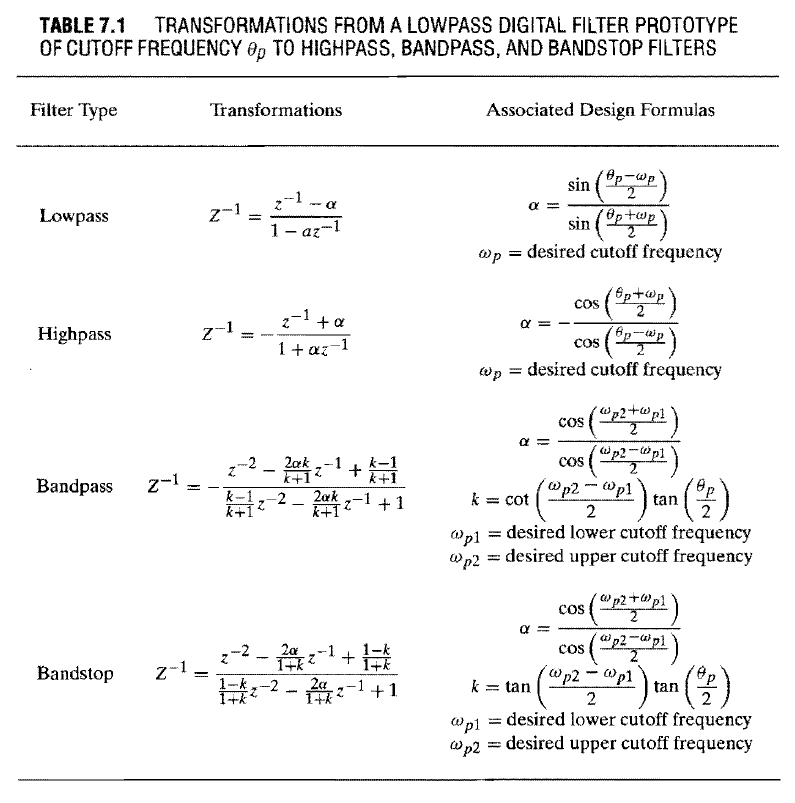
\includegraphics[scale=0.6]{figs/filter_transformation.png}
\end{frame}

\section{Design from Specifications}
\begin{frame}{Outline}
	\tableofcontents[currentsection]
\end{frame}

%
\begin{frame}{Digital FIR filter design from specifications}
	
	How to find FIR $H(z)$ such that $H(e^{j\omega})$ best approximates a desired frequency response $H_d(e^{j\omega})$? Essentially a polynomial curve fitting problem.
	\begin{center}
		\resizebox{0.6\linewidth}{!}{\begin{tikzpicture}
\begin{axis}[
name=plot1,
axis lines*=middle,
enlargelimits = upper, clip=false,
scale only axis,
axis on top=false,
axis line style={->,>=stealth},
width=0.6\textwidth,
height=0.4\textwidth,
xlabel={$\omega$},
ylabel={$H_d(e^{j\omega})$},
every axis x label/.style={
	at={(ticklabel* cs:1)},
	xshift=-0.2cm,
	anchor=north,
},
every axis y label/.style={
	at={(ticklabel* cs:1)},
	xshift=0.4cm,
	%yshift=0.35cm,
	anchor=south,
},
every outer x axis line/.append style={white!15!black},
every x tick label/.append style={font=\color{white!15!black}},
xmin=0, xmax=1,
ymin=0, ymax=1.25,
ytick={0.2, 0.9, 1.1}, yticklabels={$\delta_2$, $1-\delta_1$, $1+\delta_1$},
xtick={0, 0.25, 0.6, 1},
xticklabels ={$0$, $\omega_p$, $\omega_s$, $\pi$},
every outer y axis line/.append style={white!15!black},
every y tick label/.append style={font=\color{white!15!black}},
legend style={draw=white!15!black,fill=white,legend cell align=left}]
\addplot[solid, line width=1pt, domain=0:0.25, samples=2] {1.1}; 
\addplot[solid, line width=1pt, domain=0:0.25, samples=2] {0.9};
\addplot[solid, line width=1pt, domain=0.6:1, samples=2] {0.2};

\addplot[blue2, line width=2pt, domain=0:0.25, samples=2] {1};
\addplot[blue2, line width=2pt, domain=0.6:1, samples=2] {0};
\addplot[dashed, line width=1pt] coordinates {(0.25, 0) (0.25, 0.9)};
\addplot[dashed, line width=1pt] coordinates {(0.6, 0) (0.6, 0.9)};

\fill [black!20] (axis cs: 0, 1.1) rectangle (0.25, 1.2);
\fill [black!20] (axis cs: 0, 0.9) rectangle (0.25, 0.8);
\fill [black!20] (axis cs: 0.6, 0.2) rectangle (1, 0.3);

\node[align=center, text width = 2cm, scale=0.8] at ($(axis cs: 0, 0.5)!0.5!(axis cs: 0.25, 0.5)$) {Passband};
\node[align=center, text width = 2cm, scale=0.8] at ($(axis cs: 0.6, 0.5)!0.5!(axis cs: 1, 0.5)$) {Stopband};

\ifdefined\CARE
	\fill [red!30] (axis cs: 0.25, 0) rectangle (axis cs: 0.6, 1);
	\node[align=center, text width = 2cm, scale=0.8] at ($(axis cs: 0.25, 0.5)!0.5!(axis cs: 0.6, 0.5)$) {Don't care};
\else
	\node[align=center, text width = 2cm, scale=0.8] at ($(axis cs: 0.25, 0.5)!0.5!(axis cs: 0.6, 0.5)$) {Transition};
\fi

\end{axis}

\ifdefined\CARE
	\node[blue2, below=0.5cm, align=right, text width = 2.5cm, scale=0.8] (t1) at ($(plot1.south west)$) {$W(\omega \leq \omega_p) = 1$};
	\node[red2, below=0.5cm, right=0.01cm of t1, align=center, text width = 4cm, scale=0.8] (t2) {$W(\omega_p < \omega < \omega_s) = 0$};
	\node[blue2, below=0.5cm, right=0.01cm of t2, align=center, text width = 2.5cm, scale=0.8] (t3) {$W(\omega \geq \omega_s) = 1$};
\fi
\end{tikzpicture}}
	\end{center}
	
	\textbf{Design techniques:}
	\begin{itemize}
		\item Window method
		\item Optimal filter design
		\begin{itemize}
			\item Parks-McClellan algorithm
			\item Least squares
		\end{itemize}
	\end{itemize}
\end{frame}


\subsection{Window method}
%
\begin{frame}{Window method}

An easy way to design an FIR filter to match a desired frequency response $H_d(e^{j\omega})$ is to calculate the inverse DTFT of $H_d(e^{j\omega})$ and truncate the result to a reasonable number of samples (similar to impulse invariance):

\begin{equation}
	h_d[n] = \frac{1}{2\pi}\int_{-\pi}^{\pi}H_d(e^{j\omega})e^{j\omega n} d\omega \tag{inverse DTFT}
\end{equation}

Then we truncate it to have a most $M+1$ samples
\begin{equation}
	h[n] = \begin{cases}
	h_d[n], & n = 0, 1, \ldots, M \\
	0, & \text{otherwise}
	\end{cases} \tag{truncated sequence}
\end{equation} 

Another way to write truncation is 
\begin{equation*}
	h[n] = w[n]h_d[n], \quad\text{where}~w[n] = \begin{cases}
	1, & n = 0, 1, \ldots, M \\
	0, & \text{otherwise}
	\end{cases} \tag{truncated sequence}
\end{equation*}
$w[n]$ is the \textbf{window sequence}, which in this case is the rectangular window. 
\end{frame}

\begin{frame}{Window method}

Representing truncation as $h[n] = w[n]h_d[n]$, gives us an easy way to understand what happens in the frequency domain.
~\\
~\\

Multiplication in time domain means convolution in the frequency domain:
\begin{align*}
	H(e^{j\omega}) &= \frac{1}{2\pi}W(e^{j\omega}) \ast H_d(e^{j\omega}) \\
	& = \frac{1}{2\pi}\int_{-\pi}^{\pi} H_d(e^{j\theta})W(e^{j(\omega - \theta)})d\theta \tag{convolution}
\end{align*}

\textbf{Problem:} $H(e^{j\omega})$ will not be equal to $H_d(e^{j\omega})$. Instead, it will be a \textit{smeared} version of the desired response $H_d(e^{j\omega})$.

\end{frame}

\begin{frame}<beamer:2-|handout:2->{Revisiting the Gibbs phenomenon}

\begin{columns}[t]
	\begin{column}{0.5\linewidth}
		\textbf{Time domain}
		\vspace{0.1cm}
		\begin{equation*}
		h_{lpf}[n] = \frac{\sin\omega_cn}{\pi n} = \frac{\omega_c}{\pi}\mathrm{sinc}\Big(\frac{\omega_c}{\pi} n\Big)
		\end{equation*}
	\end{column}
	
	\begin{column}{0.5\linewidth}
		\textbf{Frequency domain}
		\vspace{-0.2cm}
		\only<1|handout:1>{
			\begin{equation*}
			H_{lpf}(e^{j\omega}) = \begin{cases}
			1, & |\omega|\leq\omega_c \\
			0, & \omega_c < |\omega|\leq \pi
			\end{cases}
			\end{equation*}	
		}
		\only<2-|handout:2->{
			\begin{equation*}
			H_{M}(e^{j\omega}) = \sum_{n=\tikz[baseline]{
					\node[fill=blue!20,anchor=base,scale=0.7] {$-M$};
			}}^{\tikz[baseline]{
					\node[fill=blue!20,anchor=base,scale=0.7] {$M$};
			}} \frac{\sin\omega_cn}{\pi n}e^{-j\omega n}
			\end{equation*}	
		}
	\end{column}
\end{columns}
\vspace{0.3cm}

\centering
\resizebox{\linewidth}{!}{\begin{tikzpicture} 
\only<1|handout:1>{
\begin{axis}[
name=ideal_lpf_td,
anchor=origin,
axis lines*=middle,
enlargelimits = true,
ymin=-0.1,
ymax=1.2*0.5,
xmin=-10,
xmax=10,
axis line style={->,>=stealth},
xlabel={$n$},
ylabel={$h_{lpf}[n]$},
yticklabel style = {yshift=0.2cm},
xticklabel style = {yshift=-0.1cm},
every axis x label/.style={
	at={(ticklabel* cs:1)},
	anchor=north,
},
every axis y label/.style={
	at={(ticklabel* cs:1)},
	anchor=south,
},
ytick=0.5,
yticklabels={$\frac{\omega_c}{\pi}$},
xtick=\empty,
every outer y axis line/.append style={white!15!black},
every y tick label/.append style={font=\color{white!15!black}},
legend style={draw=white!15!black,fill=white,legend cell align=left}]

\addplot[ycomb, mark=*, fill=white, mark options={scale=1.5, fill=white}, line width=1.5pt, domain=-10:10, samples=21] {sin(deg(pi/2*x))/(pi*x) + 1/2*(x == 0)};
\addplot[smooth, black!20, line width=1pt, domain=-10:10, samples=21] {sin(deg(pi/2*x))/(pi*x) + 1/2*(x == 0)};
\end{axis}

\begin{axis}[
name=ideal_lpf_fd,
at=(ideal_lpf_td.right of south east), anchor=left of south west,
axis lines*=middle,
enlargelimits = true,
xmax=4,
xmin=-4,
ymin=-0.2,
ymax=1.2,
axis line style={->,>=stealth},
xlabel={$\omega$},
ylabel={$H_{lpf}(e^{j\omega})$},
yticklabel style = {yshift=0.2cm},
xticklabel style = {yshift=-0.3cm},
every axis x label/.style={
    at={(ticklabel* cs:1)},
    anchor=north,
},
every axis y label/.style={
    at={(ticklabel* cs:1)},
    anchor=south,
},
xtick=\empty,
ytick={1},
xtick={-3.14, -1.5708, 1.5708, 3.14},
xticklabels={$-\pi$, $-\omega_c$, $\omega_c$, $\pi$},
every outer y axis line/.append style={white!15!black},
every y tick label/.append style={font=\color{white!15!black}},
legend style={draw=white!15!black,fill=white,legend cell align=left}]

	\addplot[black, domain=-pi/2:pi/2, samples=2,line width=2pt] {1};
	\addplot[black, line width=2pt] coordinates {(-pi/2, 0) (-pi/2, 1.01)};
	\addplot[black, domain=-pi:-pi/2, samples=2,line width=2pt] {0};
	\addplot[black, domain=pi/2:pi, samples=2,line width=2pt] {0};
	\addplot[black, line width=2pt] coordinates {(pi/2, 0) (pi/2, 1.01)};
\end{axis}
}

%%%%%%%%%%%%%%%%%% 
\only<2|handout:2>{
	\begin{axis}[
	name=truncated_lpf_td,
	anchor=origin,
	axis lines*=middle,
	enlargelimits = true,
	ymin=-0.1,
	ymax=1.2*0.5,
	xmin=-7,
	xmax=7,
	axis line style={->,>=stealth},
	xlabel={$n$},
	ylabel={$h_{lpf}[n]$},
	yticklabel style = {yshift=0.2cm},
	xticklabel style = {yshift=0.6cm},
	every axis x label/.style={
		at={(ticklabel* cs:1)},
		anchor=north,
	},
	every axis y label/.style={
		at={(ticklabel* cs:1)},
		anchor=south,
	},
	ytick=0.5,
	yticklabels={$\frac{\omega_c}{\pi}$},
	xtick={-7, 7},
	xticklabels={\tikz[baseline]{\node[fill=blue!20,anchor=base,scale=0.7] {$-M$};}, \tikz[baseline]{\node[fill=blue!20,anchor=base,scale=0.7] {$M$};}},
	every outer y axis line/.append style={white!15!black},
	every y tick label/.append style={font=\color{white!15!black}},
	legend style={draw=white!15!black,fill=white,legend cell align=left}]
	
	\addplot[ycomb, mark=*, fill=white, mark options={scale=1.5, fill=white}, line width=1.5pt, domain=-7:7, samples=15] {sin(deg(pi/2*x))/(pi*x) + 1/2*(x == 0)};
	\addplot[smooth, black!20, line width=1pt, domain=-7:7, samples=15] {sin(deg(pi/2*x))/(pi*x) + 1/2*(x == 0)};
	\end{axis}
	
	\begin{axis}[
	name=truncated_lpf_fd,
	at=(truncated_lpf_td.right of south east), anchor=left of south west,
	axis lines*=middle,
	enlargelimits = true,
	xmax=4,
	xmin=-4,
	ymin=-0.2,
	ymax=1.2,
	axis line style={->,>=stealth},
	xlabel={$\omega$},
	ylabel={$H_{lpf}(e^{j\omega})$},
	yticklabel style = {yshift=0.2cm},
	xticklabel style = {yshift=-0.3cm},
	every axis x label/.style={
		at={(ticklabel* cs:1)},
		anchor=north,
	},
	every axis y label/.style={
		at={(ticklabel* cs:1)},
		anchor=south,
	},
	xtick=\empty,
	ytick={1},
	xtick={-3.14, -1.5708, 1.5708, 3.14},
	xticklabels={$-\pi$, $-\omega_c$, $\omega_c$, $\pi$},
	every outer y axis line/.append style={white!15!black},
	every y tick label/.append style={font=\color{white!15!black}},
	legend style={draw=white!15!black,fill=white,legend cell align=left}]
	
	\addplot[black!20, domain=-pi/2:pi/2, samples=2,line width=2pt] {1};
	\addplot[black!20, line width=2pt] coordinates {(-pi/2, 0) (-pi/2, 1.01)};
	\addplot[black!20, domain=-pi:-pi/2, samples=2,line width=2pt] {0};
	\addplot[black!20, domain=pi/2:pi, samples=2,line width=2pt] {0};
	\addplot[black!20, line width=2pt] coordinates {(pi/2, 0) (pi/2, 1.01)};
	
	\addplot [color=black, solid, line width=1.5pt, forget plot]
	table[row sep=crcr]{
		-3.1416 0.039209 \\
		-3.0781 0.034184 \\
		-3.0147 0.020324 \\
		-2.9512 0.00099044 \\
		-2.8877 -0.019066 \\
		-2.8243 -0.0348 \\
		-2.7608 -0.042056 \\
		-2.6973 -0.038583 \\
		-2.6339 -0.024655 \\
		-2.5704 -0.0031491 \\
		-2.5069 0.020968 \\
		-2.4435 0.041656 \\
		-2.38 0.053128 \\
		-2.3165 0.051242 \\
		-2.2531 0.034652 \\
		-2.1896 0.0054863 \\
		-2.1261 -0.030621 \\
		-2.0627 -0.065184 \\
		-1.9992 -0.088127 \\
		-1.9357 -0.089437 \\
		-1.8723 -0.060929 \\
		-1.8088 0.0022081 \\
		-1.7453 0.10035 \\
		-1.6819 0.22911 \\
		-1.6184 0.37975 \\
		-1.5549 0.54037 \\
		-1.4915 0.69762 \\
		-1.428 0.83864 \\
		-1.3645 0.95293 \\
		-1.3011 1.0338 \\
		-1.2376 1.0793 \\
		-1.1741 1.0921 \\
		-1.1107 1.0788 \\
		-1.0472 1.0487 \\
		-0.98373 1.0122 \\
		-0.92026 0.97863 \\
		-0.8568 0.95526 \\
		-0.79333 0.94598 \\
		-0.72986 0.95114 \\
		-0.6664 0.96788 \\
		-0.60293 0.99105 \\
		-0.53947 1.0146 \\
		-0.476 1.0328 \\
		-0.41253 1.0417 \\
		-0.34907 1.0397 \\
		-0.2856 1.0278 \\
		-0.22213 1.0093 \\
		-0.15867 0.98893 \\
		-0.0952 0.97181 \\
		-0.031733 0.96207 \\
		0.031733 0.96207 \\
		0.0952 0.97181 \\
		0.15867 0.98893 \\
		0.22213 1.0093 \\
		0.2856 1.0278 \\
		0.34907 1.0397 \\
		0.41253 1.0417 \\
		0.476 1.0328 \\
		0.53947 1.0146 \\
		0.60293 0.99105 \\
		0.6664 0.96788 \\
		0.72986 0.95114 \\
		0.79333 0.94598 \\
		0.8568 0.95526 \\
		0.92026 0.97863 \\
		0.98373 1.0122 \\
		1.0472 1.0487 \\
		1.1107 1.0788 \\
		1.1741 1.0921 \\
		1.2376 1.0793 \\
		1.3011 1.0338 \\
		1.3645 0.95293 \\
		1.428 0.83864 \\
		1.4915 0.69762 \\
		1.5549 0.54037 \\
		1.6184 0.37975 \\
		1.6819 0.22911 \\
		1.7453 0.10035 \\
		1.8088 0.0022081 \\
		1.8723 -0.060929 \\
		1.9357 -0.089437 \\
		1.9992 -0.088127 \\
		2.0627 -0.065184 \\
		2.1261 -0.030621 \\
		2.1896 0.0054863 \\
		2.2531 0.034652 \\
		2.3165 0.051242 \\
		2.38 0.053128 \\
		2.4435 0.041656 \\
		2.5069 0.020968 \\
		2.5704 -0.0031491 \\
		2.6339 -0.024655 \\
		2.6973 -0.038583 \\
		2.7608 -0.042056 \\
		2.8243 -0.0348 \\
		2.8877 -0.019066 \\
		2.9512 0.00099044 \\
		3.0147 0.020324 \\
		3.0781 0.034184 \\
		3.1416 0.039209 \\
	};
	
	\node at (axis cs: 3.14, 1.1) {\Large \tikz[baseline]{
			\node[fill=blue!20,anchor=base] (t1) {$M = 7$}}};
	
	\end{axis}
}

%%%%%%%%%%%%%%%%%% 
\only<3|handout:3>{
	\begin{axis}[
	name=truncated_lpf_td,
	anchor=origin,
	axis lines*=middle,
	enlargelimits = true,
	ymin=-0.1,
	ymax=1.2*0.5,
	xmin=-19,
	xmax=19,
	axis line style={->,>=stealth},
	xlabel={$n$},
	ylabel={$h_{lpf}[n]$},
	yticklabel style = {yshift=0.2cm},
	xticklabel style = {yshift=0.6cm},
	every axis x label/.style={
		at={(ticklabel* cs:1)},
		anchor=north,
	},
	every axis y label/.style={
		at={(ticklabel* cs:1)},
		anchor=south,
	},
	ytick=0.5,
	yticklabels={$\frac{\omega_c}{\pi}$},
	xtick={-19, 19},
	xticklabels={\tikz[baseline]{\node[fill=blue!20,anchor=base,scale=0.7] {$-M$};}, \tikz[baseline]{\node[fill=blue!20,anchor=base,scale=0.7] {$M$};}},
	every outer y axis line/.append style={white!15!black},
	every y tick label/.append style={font=\color{white!15!black}},
	legend style={draw=white!15!black,fill=white,legend cell align=left}]
	
	\addplot[ycomb, mark=*, fill=white, mark options={scale=1.5, fill=white}, line width=1.5pt,  domain=-19:19, samples=39] {sin(deg(pi/2*x))/(pi*x) + 1/2*(x == 0)};
	\addplot[smooth, black!20, line width=1pt, domain=-19:19, samples=39] {sin(deg(pi/2*x))/(pi*x) + 1/2*(x == 0)};
	\end{axis}
	
	\begin{axis}[
	name=truncated_lpf_fd,
	at=(truncated_lpf_td.right of south east), anchor=left of south west,
	axis lines*=middle,
	enlargelimits = true,
	xmax=4,
	xmin=-4,
	ymin=-0.2,
	ymax=1.2,
	axis line style={->,>=stealth},
	xlabel={$\omega$},
	ylabel={$H_{lpf}(e^{j\omega})$},
	yticklabel style = {yshift=0.2cm},
	xticklabel style = {yshift=-0.3cm},
	every axis x label/.style={
		at={(ticklabel* cs:1)},
		anchor=north,
	},
	every axis y label/.style={
		at={(ticklabel* cs:1)},
		anchor=south,
	},
	xtick=\empty,
	ytick={1},
	xtick={-3.14, -1.5708, 1.5708, 3.14},
	xticklabels={$-\pi$, $-\omega_c$, $\omega_c$, $\pi$},
	every outer y axis line/.append style={white!15!black},
	every y tick label/.append style={font=\color{white!15!black}},
	legend style={draw=white!15!black,fill=white,legend cell align=left}]
	
	\addplot[black!20, domain=-pi/2:pi/2, samples=2,line width=2pt] {1};
	\addplot[black!20, line width=2pt] coordinates {(-pi/2, 0) (-pi/2, 1.01)};
	\addplot[black!20, domain=-pi:-pi/2, samples=2,line width=2pt] {0};
	\addplot[black!20, domain=pi/2:pi, samples=2,line width=2pt] {0};
	\addplot[black!20, line width=2pt] coordinates {(pi/2, 0) (pi/2, 1.01)};
	
	\addplot [color=black, solid, line width=1.5pt, forget plot]
table[row sep=crcr]{
	-3.1416 0.015876 \\
	-3.11 0.012806 \\
	-3.0784 0.0047726 \\
	-3.0469 -0.0051424 \\
	-3.0153 -0.013122 \\
	-2.9837 -0.01607 \\
	-2.9521 -0.012801 \\
	-2.9206 -0.0045107 \\
	-2.889 0.0056547 \\
	-2.8574 0.013781 \\
	-2.8259 0.016676 \\
	-2.7943 0.013113 \\
	-2.7627 0.0043342 \\
	-2.7311 -0.006365 \\
	-2.6996 -0.014863 \\
	-2.668 -0.017776 \\
	-2.6364 -0.013789 \\
	-2.6048 -0.0042266 \\
	-2.5733 0.0073679 \\
	-2.5417 0.016523 \\
	-2.5101 0.019535 \\
	-2.4785 0.014937 \\
	-2.447 0.0041704 \\
	-2.4154 -0.0088347 \\
	-2.3838 -0.019057 \\
	-2.3522 -0.022276 \\
	-2.3207 -0.016768 \\
	-2.2891 -0.004133 \\
	-2.2575 0.011106 \\
	-2.226 0.023056 \\
	-2.1944 0.026652 \\
	-2.1628 0.019706 \\
	-2.1312 0.0040161 \\
	-2.0997 -0.01496 \\
	-2.0681 -0.029875 \\
	-2.0365 -0.034159 \\
	-2.0049 -0.024686 \\
	-1.9734 -0.0034348 \\
	-1.9418 0.022586 \\
	-1.9102 0.043309 \\
	-1.8786 0.049014 \\
	-1.8471 0.034142 \\
	-1.8155 0.00025733 \\
	-1.7839 -0.042935 \\
	-1.7523 -0.079062 \\
	-1.7208 -0.08885 \\
	-1.6892 -0.055218 \\
	-1.6576 0.031713 \\
	-1.6261 0.1712 \\
	-1.5945 0.35111 \\
	-1.5629 0.55018 \\
	-1.5313 0.74274 \\
	-1.4998 0.90461 \\
	-1.4682 1.0186 \\
	-1.4366 1.0783 \\
	-1.405 1.0884 \\
	-1.3735 1.0631 \\
	-1.3419 1.0211 \\
	-1.3103 0.98084 \\
	-1.2787 0.95576 \\
	-1.2472 0.95147 \\
	-1.2156 0.96573 \\
	-1.184 0.99043 \\
	-1.1524 1.0152 \\
	-1.1209 1.0311 \\
	-1.0893 1.0336 \\
	-1.0577 1.0234 \\
	-1.0261 1.0055 \\
	-0.99457 0.98732 \\
	-0.963 0.97552 \\
	-0.93143 0.97388 \\
	-0.89985 0.98214 \\
	-0.86828 0.99648 \\
	-0.83671 1.0111 \\
	-0.80513 1.0206 \\
	-0.77356 1.0217 \\
	-0.74198 1.0146 \\
	-0.71041 1.0024 \\
	-0.67884 0.98987 \\
	-0.64726 0.98183 \\
	-0.61569 0.98105 \\
	-0.58412 0.98748 \\
	-0.55254 0.99841 \\
	-0.52097 1.0095 \\
	-0.48939 1.0166 \\
	-0.45782 1.0172 \\
	-0.42625 1.0111 \\
	-0.39467 1.001 \\
	-0.3631 0.99079 \\
	-0.33152 0.98432 \\
	-0.29995 0.98398 \\
	-0.26838 0.98979 \\
	-0.2368 0.99942 \\
	-0.20523 1.0091 \\
	-0.17366 1.0152 \\
	-0.14208 1.0154 \\
	-0.11051 1.0096 \\
	-0.078934 1.0002 \\
	-0.047361 0.99075 \\
	-0.015787 0.98491 \\
	0.015787 0.98491 \\
	0.047361 0.99075 \\
	0.078934 1.0002 \\
	0.11051 1.0096 \\
	0.14208 1.0154 \\
	0.17366 1.0152 \\
	0.20523 1.0091 \\
	0.2368 0.99942 \\
	0.26838 0.98979 \\
	0.29995 0.98398 \\
	0.33152 0.98432 \\
	0.3631 0.99079 \\
	0.39467 1.001 \\
	0.42625 1.0111 \\
	0.45782 1.0172 \\
	0.48939 1.0166 \\
	0.52097 1.0095 \\
	0.55254 0.99841 \\
	0.58412 0.98748 \\
	0.61569 0.98105 \\
	0.64726 0.98183 \\
	0.67884 0.98987 \\
	0.71041 1.0024 \\
	0.74198 1.0146 \\
	0.77356 1.0217 \\
	0.80513 1.0206 \\
	0.83671 1.0111 \\
	0.86828 0.99648 \\
	0.89985 0.98214 \\
	0.93143 0.97388 \\
	0.963 0.97552 \\
	0.99457 0.98732 \\
	1.0261 1.0055 \\
	1.0577 1.0234 \\
	1.0893 1.0336 \\
	1.1209 1.0311 \\
	1.1524 1.0152 \\
	1.184 0.99043 \\
	1.2156 0.96573 \\
	1.2472 0.95147 \\
	1.2787 0.95576 \\
	1.3103 0.98084 \\
	1.3419 1.0211 \\
	1.3735 1.0631 \\
	1.405 1.0884 \\
	1.4366 1.0783 \\
	1.4682 1.0186 \\
	1.4998 0.90461 \\
	1.5313 0.74274 \\
	1.5629 0.55018 \\
	1.5945 0.35111 \\
	1.6261 0.1712 \\
	1.6576 0.031713 \\
	1.6892 -0.055218 \\
	1.7208 -0.08885 \\
	1.7523 -0.079062 \\
	1.7839 -0.042935 \\
	1.8155 0.00025733 \\
	1.8471 0.034142 \\
	1.8786 0.049014 \\
	1.9102 0.043309 \\
	1.9418 0.022586 \\
	1.9734 -0.0034348 \\
	2.0049 -0.024686 \\
	2.0365 -0.034159 \\
	2.0681 -0.029875 \\
	2.0997 -0.01496 \\
	2.1312 0.0040161 \\
	2.1628 0.019706 \\
	2.1944 0.026652 \\
	2.226 0.023056 \\
	2.2575 0.011106 \\
	2.2891 -0.004133 \\
	2.3207 -0.016768 \\
	2.3522 -0.022276 \\
	2.3838 -0.019057 \\
	2.4154 -0.0088347 \\
	2.447 0.0041704 \\
	2.4785 0.014937 \\
	2.5101 0.019535 \\
	2.5417 0.016523 \\
	2.5733 0.0073679 \\
	2.6048 -0.0042266 \\
	2.6364 -0.013789 \\
	2.668 -0.017776 \\
	2.6996 -0.014863 \\
	2.7311 -0.006365 \\
	2.7627 0.0043342 \\
	2.7943 0.013113 \\
	2.8259 0.016676 \\
	2.8574 0.013781 \\
	2.889 0.0056547 \\
	2.9206 -0.0045107 \\
	2.9521 -0.012801 \\
	2.9837 -0.01607 \\
	3.0153 -0.013122 \\
	3.0469 -0.0051424 \\
	3.0784 0.0047726 \\
	3.11 0.012806 \\
	3.1416 0.015876 \\
};
	
	\node at (axis cs: 3.14, 1.1) {\Large \tikz[baseline]{
			\node[fill=blue!20,anchor=base] (t1) {$M = 19$}}};
	
	\end{axis}
}

\end{tikzpicture}}
\end{frame}

\begin{frame}{Revisiting the Gibbs phenomenon}
\begin{itemize}
	\item The Gibbs phenomenon appears when we truncate the impulse response of the ideal lowpass filter (or any discontinuous DTFT). 
	\item In lecture 1, we attributed this to convergence issues of the DTFT for non-absolute summable sequences. The DTFT of the sinc converges only in the mean square sense, and not uniformly
	\item Another way to view the Gibbs phenomenon is as a result of windowing.
\begin{align*}
H(e^{j\omega}) &= \frac{1}{2\pi}W(e^{j\omega}) \ast H_d(e^{j\omega}) \tag{convolution}
\end{align*}
	\item In this case the desired response $H_d(e^{j\omega})$ is the ideal lowpass filter, and the window function is
	\begin{align*}
	&w[n] = \begin{cases}
	1, & n = -M, -M+1, \ldots, M-1, M \\
	0, & \text{otherwise} 
	\end{cases} \\
	&\Longleftrightarrow W(e^{j\omega}) = \frac{\sin(\omega(2M+1)/2)}{\sin(\omega/2)}
	\end{align*}
\end{itemize}
\end{frame}

\begin{frame}{Rectangular window}
\begin{center}
	\resizebox{0.6\linewidth}{!}{\begin{tikzpicture}
\begin{axis}[
name=plot2,
%at=(plot1.below south east), anchor=above north east, xshift=1cm,
axis lines*=middle,
enlargelimits = upper, clip=true,
scale only axis,
axis line style={->,>=stealth, shorten >= 0pt},
xlabel={$\omega$},
ylabel={$W(e^{j\omega})$},
every axis x label/.style={
	at={(ticklabel* cs:1)},
	xshift=-0.2cm,
	anchor=north,
},
every axis y label/.style={
	at={(ticklabel* cs:1)},
	xshift=0.4cm,
	anchor=south,
},
every outer x axis line/.append style={white!15!black},
every x tick label/.append style={font=\color{white!15!black}},
xmin=-1, xmax=1,
ymin=-0.25, ymax=1,
xtick={-1, -0.5, 0, 0.5, 1},
xticklabels ={$-\pi$, $-\pi/2$, $0$,  $\pi/2$, $\pi$},
ytick=\empty,
every outer y axis line/.append style={white!15!black},
every y tick label/.append style={font=\color{white!15!black}},
legend style={draw=white!15!black,fill=white,legend cell align=left}]

\only<1|handout:1>{
\def\M{7}
\addplot [smooth, color=black, solid, line width=2pt, domain=-1:1, samples=100] {1/(2*\M+1)*sin(deg(pi*x*(2*\M+1)/2))/sin(deg(pi*x/2))}; \addlegendentry{$M = 7$};
}

\only<2|handout:1>{
\def\M{19}
\addplot [smooth, color=blue2, solid, line width=2pt, domain=-1:1, samples=200] {1/(2*\M+1)*sin(deg(pi*x*(2*\M+1)/2))/sin(deg(pi*x/2))}; \addlegendentry{$M = 19$};
}
\end{axis}
\end{tikzpicture}}
\end{center}

The large sidelobes of $W(e^{j\omega})$ cause \textit{ringing} (Gibbs phenomenon) in the frequency response of $H(e^{j\omega})$ near discontinuities of $H_d(e^{j\omega})$.

To minimize the \textit{ringing}, the sidelobes have to be small. 
\end{frame}

\begin{frame}{Rectangular window}

From Fourier transform theory, we can show that the rectangular window produces $H(e^{j\omega})$ that \underline{best} matches $H_d(e^{j\omega})$ in the mean-square sense. That is,

\begin{equation*}
\frac{1}{2\pi}\int_{-\pi}^{\pi}|H(e^{j\omega}) - H_d(e^{j\omega})|^2d\omega, \tag{mean-square error}
\end{equation*}
is \underline{minimized} when $w[n]$ is the rectangular window.

\textbf{Question:} are there other windows $w[n]$ that minimize issues with discontinuities without excessively increasing the mean-square error?
\end{frame}

%
\begin{frame}{Commonly used windows} \fontsize{10pt}{10}\selectfont
\textbf{Rectangular:}
\begin{equation*}
w[n] = \begin{cases}
1, &0 \leq n \leq M \\
0, &\text{otherwise}
\end{cases}
\end{equation*}

\textbf{Bartlett (triangular):}
\begin{equation*}
w[n] = \begin{cases}
2n/M, & 0 \leq n \leq M/2, M \text{ even}\\
2 - 2n/M, & M/2 < n \leq M \\
0, & \text{otherwise}
\end{cases}
\end{equation*}

\textbf{Hann:}
\begin{equation*}
w[n] = \begin{cases}
0.5 - 0.5\cos(2\pi n/M), & 0 \leq n \leq M, \\
0, &\text{otherwise}
\end{cases}
\end{equation*}

\textbf{Hamming:}
\begin{equation*}
w[n] = \begin{cases}
0.54 - 0.46\cos(2\pi n/M), & 0 \leq n \leq M, \\
0, &\text{otherwise}
\end{cases}
\end{equation*}

\textbf{Blackman:}
\begin{equation*}
w[n] = \begin{cases}
0.42 - 0.5\cos(2\pi n/M) + 0.08\cos(4\pi n/M), & 0 \leq n \leq M, \\
0, &\text{otherwise}
\end{cases}
\end{equation*}
\end{frame}

%
\begin{frame}{Commonly used windows}
\textbf{Time domain}

All windows are symmetric about $M/2$.

\begin{center}
\resizebox{0.9\textwidth}{!}{\def\M{10} % window length
\begin{tikzpicture}
\begin{axis}[
%at=(plot1.below south east), anchor=above north east, xshift=1cm,
axis lines*=middle,
enlargelimits = upper, clip=false,
scale only axis,
width=\textwidth,
height=0.5\textwidth,
axis line style={->,>=stealth, shorten >= 0pt},
xlabel={$n$},
ylabel={$w[n]$},
every axis x label/.style={
	at={(ticklabel* cs:1)},
	xshift=-0.2cm,
	anchor=north,
},
every axis y label/.style={
	at={(ticklabel* cs:1)},
	xshift=0.4cm,
	anchor=south,
},
every outer x axis line/.append style={white!15!black},
every x tick label/.append style={font=\color{white!15!black}},
xmin=0, xmax=\M,
ymin=0, ymax=1,
xtick={0, 5, \M},
xticklabels ={$0$, $\frac{M}{2}$, $M$},
ytick=1,
every outer y axis line/.append style={white!15!black},
every y tick label/.append style={font=\color{white!15!black}},
legend style={draw=white!15!black,fill=white,legend cell align=left, at={(axis cs: 1.05, -5)}}]
\addplot [smooth, color=black, solid, line width=1.5pt, domain=0:\M, samples=2] {1} node[pos=0.8, black, pin={[pin edge={black, thick}]30:{Rectangular}}, inner sep=0pt] {};

\addplot [smooth, color=blue2, solid, line width=1.5pt, domain=0:\M/2, samples=21] {2*x/\M};
\addplot [smooth, color=blue2, solid, line width=1.5pt, domain=\M/2:\M, samples=21] {2-2*x/\M} node[pos=0.75, blue2, pin={[pin edge={blue2, thick}]30:{Bartlett (triangular)}}, inner sep=0pt] {};

\addplot [smooth, color=green2, solid, line width=1.5pt, domain=0:\M, samples=21] {0.5-0.5*cos(deg(2*pi*x/\M))} node[pos=0.78, green2, pin={[pin edge={green2, thick}]30:{Hann}}, inner sep=0pt] {};

\addplot [smooth, color=orange2, solid, line width=1.5pt, domain=0:\M, samples=21] {0.54-0.46*cos(deg(2*pi*x/\M))} node[pos=0.75, orange2, pin={[pin edge={orange2, thick}]30:{Hamming}}, inner sep=0pt] {};

\addplot [smooth, color=red2, solid, line width=1.5pt, domain=0:\M, samples=21] {0.42-0.5*cos(deg(2*pi*x/\M)) + 0.08*cos(deg(4*pi*x/\M))} node[pos=0.65, red2, pin={[pin edge={red2, thick}]30:{Blackman}}, inner sep=0pt] {};

\end{axis}
\end{tikzpicture}}
\end{center}
\textbf{Note:} $n$ is discrete. These curves were plotted as continuous functions just for easier visualization.

We will revisit windows when talking about spectrum analysis (lecture 12)
\end{frame}

%
\begin{frame}{Linear phase in filters designed by windowing}
	If the window is causal and symmetric \underline{and} if the desired impulse response $h_d[n]$ is causal and symmetric, then it follows
	\begin{align}
		w[n] &= \pm w[M-n] \tag{causal and symmetric window} \\
		h_d[n] &= \pm h_d[M-n] \tag{causal and symmetric $h_d[n]$} \\
		h[n] = w[n]h_d[n] &= \pm w[M-n]h_d[M-n] = \pm h[M-n] \tag{causal and symmetric $h[n]$}
	\end{align}
	
	Therefore, $h[n]$ is either even or odd symmetric and consequently $H(e^{j\omega})$ has generalized linear phase.
	
\end{frame}

%
\begin{frame}{Kaiser window}

It's typically desired that the window be maximally concentrated around $\omega = 0$ (small sidelobe area).

The \textbf{Kaiser window} is a nearly optimal choice

\begin{equation*}
	w[n] = \begin{cases}
	\displaystyle\frac{I_0\Big(\beta\sqrt{1- (n-M/2)^2/(M/2)^2}\Big)}{I_0(\beta)}, & 0 \leq n \leq M \\
	0, & \text{otherwise}
	\end{cases},
\end{equation*}
where $\beta$ is a design parameter, and $I_0(\cdot)$ is the \textbf{modified Bessel function of first kind}.

See section 7.5.3 of the textbook for recommendations on values of $\beta$ for lowpass filter design.

\end{frame}

%
\begin{frame}{Summary on FIR filter design by the window method}
	\begin{enumerate}
		\item From the desired frequency response $H_d(e^{j\omega})$ calculate the desired impulse response $h_d[n]$.
		\item Choose the filter order $M$ and the window $w[n]$. Then,
		\begin{equation*}
			h[n] = \begin{cases}
			h_d[n]w[n], & n = 0, \ldots, M \\
			0, &\text{otherwise}
			\end{cases}
		\end{equation*}
		Kaiser window depends on parameters $\beta$ and $M$. Other windows only depend on $M$.
		
		\item Linear phase is guaranteed by selecting causal and symmetric window $w[n]$ and desired impulse response $h_d[n]$
	\end{enumerate}

In Matlab: 

\texttt{fir1} uses Hamming window by default. Other windows can be passed as parameters:
\begin{equation*}
\texttt{>> fir1(M, wc/pi, `lowpass', kaiser(M+1, beta))}
\end{equation*} 
designs a lowpass FIR filter of order $M$ and cutoff frequency $\omega_c$ using the window method with Kaiser window with parameter $\beta$



\end{frame}

\subsection{Optimal FIR filter design}
\begin{frame}<beamer:1|handout:0>{Outline}
	\tableofcontents[currentsubsection]
\end{frame}

\begin{frame}{Optimal FIR filter design}
\begin{itemize}
	\item Though straightforward, filter design by windowing is \underline{sub-optimal} in the sense that it compromises accuracy for better \textit{handling} of discontinuities in $H_d(e^{j\omega})$.
	\item More importantly, there was no well-defined metric to evaluate filters
\end{itemize}
	\vspace{0.25cm}
	
	A sensible choice for evaluation metric is the \textbf{weighted error}:
	\begin{align*}
		E(\omega) = W(\omega)\Big(H_d(e^{j\omega}) - H(e^{j\omega})\Big), \tag{weighted error}
	\end{align*}
	where $0 \leq W(\omega) \leq 1$ is the \textbf{weight function}. 
	\vspace{0.25cm}
	
	\begin{itemize}
		\item Generally, we choose either $W(\omega) = 1$ or $W(\omega) = 0$ over a certain frequency band.
		\item Making $W(\omega) = 0$ over a certain band means that we don't care about the error in that band. Generally, we choose $W(\omega) = 0$ around discontinuities of $H_d(e^{j\omega})$ i.e., transition bands.
	\end{itemize}	
\end{frame}

\begin{frame}{Optimal FIR filter design}

	\textbf{Example:}
		
	\begin{center}
		\def\CARE{1}
		\resizebox{0.9\linewidth}{!}{\begin{tikzpicture}
\begin{axis}[
name=plot1,
axis lines*=middle,
enlargelimits = upper, clip=false,
scale only axis,
axis on top=false,
axis line style={->,>=stealth},
width=0.6\textwidth,
height=0.4\textwidth,
xlabel={$\omega$},
ylabel={$H_d(e^{j\omega})$},
every axis x label/.style={
	at={(ticklabel* cs:1)},
	xshift=-0.2cm,
	anchor=north,
},
every axis y label/.style={
	at={(ticklabel* cs:1)},
	xshift=0.4cm,
	%yshift=0.35cm,
	anchor=south,
},
every outer x axis line/.append style={white!15!black},
every x tick label/.append style={font=\color{white!15!black}},
xmin=0, xmax=1,
ymin=0, ymax=1.25,
ytick={0.2, 0.9, 1.1}, yticklabels={$\delta_2$, $1-\delta_1$, $1+\delta_1$},
xtick={0, 0.25, 0.6, 1},
xticklabels ={$0$, $\omega_p$, $\omega_s$, $\pi$},
every outer y axis line/.append style={white!15!black},
every y tick label/.append style={font=\color{white!15!black}},
legend style={draw=white!15!black,fill=white,legend cell align=left}]
\addplot[solid, line width=1pt, domain=0:0.25, samples=2] {1.1}; 
\addplot[solid, line width=1pt, domain=0:0.25, samples=2] {0.9};
\addplot[solid, line width=1pt, domain=0.6:1, samples=2] {0.2};

\addplot[blue2, line width=2pt, domain=0:0.25, samples=2] {1};
\addplot[blue2, line width=2pt, domain=0.6:1, samples=2] {0};
\addplot[dashed, line width=1pt] coordinates {(0.25, 0) (0.25, 0.9)};
\addplot[dashed, line width=1pt] coordinates {(0.6, 0) (0.6, 0.9)};

\fill [black!20] (axis cs: 0, 1.1) rectangle (0.25, 1.2);
\fill [black!20] (axis cs: 0, 0.9) rectangle (0.25, 0.8);
\fill [black!20] (axis cs: 0.6, 0.2) rectangle (1, 0.3);

\node[align=center, text width = 2cm, scale=0.8] at ($(axis cs: 0, 0.5)!0.5!(axis cs: 0.25, 0.5)$) {Passband};
\node[align=center, text width = 2cm, scale=0.8] at ($(axis cs: 0.6, 0.5)!0.5!(axis cs: 1, 0.5)$) {Stopband};

\ifdefined\CARE
	\fill [red!30] (axis cs: 0.25, 0) rectangle (axis cs: 0.6, 1);
	\node[align=center, text width = 2cm, scale=0.8] at ($(axis cs: 0.25, 0.5)!0.5!(axis cs: 0.6, 0.5)$) {Don't care};
\else
	\node[align=center, text width = 2cm, scale=0.8] at ($(axis cs: 0.25, 0.5)!0.5!(axis cs: 0.6, 0.5)$) {Transition};
\fi

\end{axis}

\ifdefined\CARE
	\node[blue2, below=0.5cm, align=right, text width = 2.5cm, scale=0.8] (t1) at ($(plot1.south west)$) {$W(\omega \leq \omega_p) = 1$};
	\node[red2, below=0.5cm, right=0.01cm of t1, align=center, text width = 4cm, scale=0.8] (t2) {$W(\omega_p < \omega < \omega_s) = 0$};
	\node[blue2, below=0.5cm, right=0.01cm of t2, align=center, text width = 2.5cm, scale=0.8] (t3) {$W(\omega \geq \omega_s) = 1$};
\fi
\end{tikzpicture}}
	\end{center}
\end{frame}

\begin{frame}{Matrix notation}
	It is hard to build efficient algorithms to deal with continuous $\omega$.
	
	We will \textit{sample} the weighted error $E(\omega)$ for a set of $N$ frequencies $\{\omega_1, \ldots, \omega_N\}$ and write everything in matrix notation:
	
	\begin{align*}
		E(\omega) &= W(\omega)\Big(H_d(e^{j\omega}) - H(e^{j\omega})\Big) \tag{continuous weighted error} \\
		e &= W(d - Qh) \tag{matrix notation}
	\end{align*}
	
	\begin{itemize}
		\item $e$ is the error vector $e_i = E(\omega_i)$
		\item $W$ is the weight matrix: $W = \text{\textbf{diag}}(w)$, where $w$ is the weight vector: $w_i = W(\omega_i)$
		\item $d$ is the desired frequency response vector: $d_i =H_d(e^{j\omega_i})$
		\item $h$ is the FIR filter coefficients vector $h_i = h[i]$. This is the vector we want to find. 
		
		\textbf{Note:} If the filter has linear phase, $h[n]$ is symmetric, so we only need to compute the coefficients $h[0], \ldots, h[\lfloor M/2\rfloor]$
	\end{itemize}
\end{frame}

\begin{frame}{Matrix notation}
	\begin{itemize}
		\item $Q$ is the matrix:
	\end{itemize}
		\begin{equation*}
			Q = \begin{bmatrix}
			2\cos(\omega_1(\frac{M}{2})) & 2\cos(\omega_1(\frac{M}{2}-1)) &\ldots & 2\cos(\omega_1) & 1 \\
			2\cos(\omega_2(\frac{M}{2})) & 2\cos(\omega_2(\frac{M}{2}-1)) & \ldots & 2\cos(\omega_2) & 1 \\
			\vdots & \vdots & \ddots & \vdots & \vdots \\
			2\cos(\omega_N(\frac{M}{2})) & 2\cos(\omega_N(\frac{M}{2}-1)) & \ldots & 2\cos(\omega_N) & 1	\\		
			\end{bmatrix}_{N\times \frac{M}{2} + 1}
		\end{equation*}
		for $h[n]$ \underline{even symmetric} and $M$ \underline{even}.
		
		This comes from the relation
		\begin{equation*}
		H(e^{j\omega}) = \sum_{m = 0}^{M}h[m]e^{j\omega m} = e^{-j\omega\frac{M}{2}}\bigg(1 + \displaystyle\sum_{n = 0}^{\frac{M}{2}-1}2h[n]\cos(\omega(M/2-n))\bigg). \tag{DTFT of symmetryic FIR $h[n]$}
		\end{equation*}

		\vspace{0.25cm}
		\textbf{Note:} in matrix $Q$ we have disregarded the term $e^{j\omega M/2}$. This way matrix $Q$ will be \underline{purely real}. Ignoring the terms $e^{j\omega M/2}$ is equivalent to disregarding the constraint that the filter must be causal. This is not a problem because we can always time-shift the result and make it causal.
		\pause 
		\textbf{Questions:} how would matrix $Q$ change for $h[n]$ even symmetric and $M$ odd? What about $h[n]$ odd symmetric?
\end{frame}

\begin{frame}{Generalized linear phase in optimal FIR filter design}
	
	\begin{block}{Even symmetry $h[n] = h[M-n]$}
		\vspace{-0.5cm}
		\begin{equation*}
		H(e^{j\omega}) = \begin{cases}
		e^{-j\omega\frac{M}{2}}\bigg(1 + \displaystyle\sum_{n = 0}^{\frac{M}{2}-1}2h[n]\cos(\omega(M/2-n))\bigg), & M~\text{even} \\
		e^{-j\omega\frac{M}{2}}\displaystyle\sum_{n = 0}^{\frac{M-1}{2}}2h[n]\cos(\omega(M/2-n)), & M~\text{odd} 
		\end{cases}
		\end{equation*}
	\end{block}
	\vspace{-0.25cm}
	\begin{block}{Odd symmetry $h[n] = -h[M-n]$}
		\vspace{-0.5cm}
		\begin{equation*}
		H(e^{j\omega}) = \begin{cases}
		e^{-j\omega \frac{M}{2}}\bigg(1 + \displaystyle\sum_{n = 0}^{\frac{M}{2}-1}2jh[n]\sin(\omega(M/2-n))\bigg), & M~\text{even} \\
		e^{-j\omega \frac{M}{2}}\displaystyle\sum_{n = 0}^{\frac{M-1}{2}}2jh[n]\sin(\omega(M/2-n)), & M~\text{odd} 
		\end{cases}
		\end{equation*}
	\end{block}
\end{frame}


\begin{frame}{Optimal FIR filter design}
	\textbf{Question:} how to find the coefficients $h[0], \ldots, h[\lfloor\frac{M}{2}\rfloor]$ (the vector $h$)?
	\vspace{0.25cm}
	
	\textbf{Two algorithms:}
	\begin{enumerate}
		\item Parks-McClellan algorithm: minimizes the maximum weighted error 
		\begin{align*}
		\min_{h[n]} &\max_\omega E(\omega) \tag{min-max problem} \\
		\min_{h} &\max_i |e_i| \tag{in matrix notation}
		\end{align*}
		\texttt{firpm} in Matlab.
		\item Least squares: minimizes the mean-square weighted error 
		\begin{align*}
		\min_{h[n]} &\frac{1}{2\pi}\int_{-\pi}^{\pi} |E(\omega)|^2d\omega \tag{least squares}\\
		\min_{h} &||e||_2^2 \tag{in matrix notation}
		\end{align*}
		\texttt{firls} in Matlab.
	\end{enumerate}
\end{frame}


\subsubsection{Parks-McClellan Algorithm}
\begin{frame}{Parks-McClellan algorithm} 
The \textbf{Parks-McClellan algorithm} finds the filter coefficients that minimize the maximum weighted error:

\begin{align*}
	\min_{h[n]} &\max_\omega E(\omega) \tag{min-max problem} \\
	\min_{h} &\max_i |e_i| \tag{in matrix notation}
\end{align*}

\begin{itemize}
	\item This problem is also known as the Chebyshev approximation problem
	\item Traditionally, this problem is solved by using the \textbf{alternation theorem} and the \textbf{Remez exchange} algorithm to iteratively find the impulse response that minimizes the maximum weighted error over a set of closed intervals in the frequency domain.
	\item We can also recast this problem as a \textbf{linear program} and use standard convex optimization packages to solve it.
\end{itemize}

\end{frame}

\begin{frame}{Parks-McClellan algorithm as a linear program} 

\begin{equation*}
\min_{h}\max_i |e_i| \tag{min-max problem}
\end{equation*}

We can rewrite this optimization problem as
\vspace{-0.1cm}
\begin{alignat*}{2}
&\min_{u} &&u  \\
&\text{subject to} \quad -&&u \leq e_i \leq u, \quad i = 1, \ldots, N \tag{equivalent linear program}
\end{alignat*}
$u$ is just a dummy scalar variable, and $e = W(d - Qh)$.
\vspace{0.2cm}

In \href{http://cvxr.com/cvx/}{CVX} for Matlab:
\begin{alignat*}{3}
\texttt{cvx\_begin} \\
	&\texttt{variable u(1)} \\
	&\texttt{variable h(floor(M/2)+1)} \\
	&\texttt{minimize u}\\
	&\texttt{subject to -u <= W*(d - Q*h) <= u} \\
\texttt{cvx\_end}
\end{alignat*}
It will return \texttt{u} and the vector \texttt{h}, which is what we really want. \end{frame}

\subsubsection{Least-squares Algorithm}
\begin{frame}{Least-squares algorithm}
The \textbf{least-squares algorithm} finds the filter coefficients that minimize the mean-square weighted error:

\begin{align*}
\min_{h[n]} \quad&\frac{1}{2\pi}\int_{-\pi}^{\pi} |E(\omega)|^2d\omega \tag{mean square weighted error}\\
\min_{h}\quad &||W(d - Qh)||_2^2 \tag{in matrix notation} \\
\min_{h} \quad&||Ah - b||_2^2 \tag{change of variables $A = WQ$ and $b = Wd$}
\end{align*}

Problems of the form $\min_h ||Ah - b||_2^2$ are referred to as \textbf{least-squares problems} and they have analytical solution:

\begin{equation*}
	h = A^\dagger b \tag{least-squares solution}
\end{equation*}
$A^\dagger = (A^HA)^{-1}A^H$ is the \textbf{Moore-Penrose pseudoinverse} (\texttt{pinv} in Matlab). 

\textbf{Note:} $A^H = (A^*)^T$ is the \textbf{Hermitian} (conjugate transpose matrix), since $A$ could be complex.
\end{frame}

%
\subsection{Examples}
\begin{frame}{Example: optimal bandpass FIR design}
	We want to design an FIR bandpass filter with the following desired response $H_d(e^{j\omega})$

	The weight function is zero in the {\color{red!50} \textbf{transition bands}}. Hence, we don't care about the error in those regions.
	
	\begin{center}
		\resizebox{0.7\textwidth}{!}{\begin{tikzpicture}
\begin{axis}[
name=plot1,
axis lines*=middle,
enlargelimits = upper, clip=false,
scale only axis,
axis on top=false,
axis line style={->,>=stealth},
width=0.6\textwidth,
height=0.4\textwidth,
xlabel={$\omega$},
ylabel={$H_d(e^{j\omega})$},
every axis x label/.style={
	at={(ticklabel* cs:1)},
	xshift=-0.2cm,
	anchor=north,
},
every axis y label/.style={
	at={(ticklabel* cs:1)},
	xshift=0.4cm,
	%yshift=0.35cm,
	anchor=south,
},
every outer x axis line/.append style={white!15!black},
every x tick label/.append style={font=\color{white!15!black}},
xmin=0, xmax=1,
ymin=0, ymax=1.25,
ytick={1},
xtick={0, 0.5, 0.7, 1},
xticklabels ={$0$, $0.5\pi$, $0.7\pi$, $\pi$},
every outer y axis line/.append style={white!15!black},
every y tick label/.append style={font=\color{white!15!black}},
legend style={draw=white!15!black,fill=white,legend cell align=left}]
\addplot[solid, blue2, line width=2pt, domain=0.5:0.7, samples=2] {1}; 
\addplot[solid, blue2, line width=2pt, domain=0:0.4, samples=2] {0}; 
\addplot[solid, blue2, line width=2pt, domain=0.8:1, samples=2] {0}; 

\fill [red!30] (axis cs: 0.4, 0) rectangle (axis cs: 0.5, 1);
\fill [red!30] (axis cs: 0.7, 0) rectangle (axis cs: 0.8, 1);
\node[red2, fill=red!30] at (axis cs: 0.8, 1.2) {$W(\omega) = 0$};
\draw[red2, <->] (axis cs: 0.7, 0.5) to (axis cs: 0.8, 0.5); 
\draw[red2, <->] (axis cs: 0.4, 0.5) to (axis cs: 0.5, 0.5);
\node[red2, above, align=center] at (axis cs: 0.45, 0.5) {$\Delta\omega$};
\node[red2, above, align=center] at (axis cs: 0.75, 0.5) {$\Delta\omega$};
\end{axis}

\end{tikzpicture}}
	\end{center}
	
	See code on Canvas/Files/Matlab/optimal\_fir\_design\_example.m.
\end{frame}

%
\begin{frame}{Non-linear phase FIR filter design using least squares}
	Many applications do not require linear phase FIR filters. In fact, in some applications the filter must have non-linear phase e.g., linear equalization (HW\#5)
	
	To design non-linear phase FIR filters using the least-squares algorithm, we just need to redefine matrix $Q$: 
	
	\begin{equation*}
		Q = \begin{bmatrix}
		1 & e^{-j\omega_1} & e^{-j2\omega_1} & \ldots & e^{-jM\omega_1} \\
		1 & e^{-j\omega_2} & e^{-j2\omega_2} & \ldots & e^{-jM\omega_2} \\
		\vdots & \vdots &  \vdots & \ddots & \vdots \\
		1 & e^{-j\omega_N} & e^{-j2\omega_N} & \ldots & e^{-jM\omega_N}
		\end{bmatrix}_{N\times M+1}
	\end{equation*}
	where $\omega_1, \ldots, \omega_N$ are evenly spaced frequencies in the interval $[-\pi, \pi]$.
	
	Note that
	\begin{equation*}
		(Qh)_k = \sum_{m = 0}^{M}h[m]e^{-j\omega_km} = H(e^{j\omega_km}) \tag{the DTFT of $h[m]$ at frequency $\omega_k$}
	\end{equation*}	
	
	Therefore, the matrix-vector product $Qh$ gives $H(e^{j\omega})$ at $N$ frequencies $\omega_1, \ldots, \omega_N$.
\end{frame}

%
\begin{frame}{Non-linear phase FIR filter design using least squares}
Now that we have the redefined matrix $Q$, we can apply the least-squares algorithm as usual

\begin{align*}
	h &= A^{\dagger}b \tag{least squares solution} \\
	\text{where } & A = WQ \text{ and } b = Wd. 
\end{align*}

\textbf{Important:} $d$ and $W$ have to be defined for the same frequencies used in calculating $Q$.

If $H_d(e^{j\omega})$ is \textbf{Hermitian symmetric} i.e., $H_d(e^{j\omega}) = H_d^*(e^{-j\omega})$, then $h$ will be purely real.

\end{frame}

%
\begin{frame}{Example: predicting band-limited signals}

\textbf{Question:} how to predict the next sample from previous samples?

\begin{center}
	\resizebox{0.7\textwidth}{!}{\begin{tikzpicture}
\begin{axis}[
name=plot2,
%at=(plot1.below south east), anchor=above north east, xshift=1cm,
axis lines*=middle,
enlargelimits = true, clip=false,
scale only axis,
axis line style={->,>=stealth, shorten >= 0pt},
xlabel={$n$},
ylabel={$x[n]$},
every axis x label/.style={
	at={(ticklabel* cs:1)},
	xshift=-0.2cm,
	anchor=north,
},
every axis y label/.style={
	at={(ticklabel* cs:1)},
	xshift=0.4cm,
	anchor=south,
},
every outer x axis line/.append style={white!15!black},
every x tick label/.append style={font=\color{white!15!black}},
xmin=0, xmax=12,
ymin=-2, ymax=2,
xtick={0, ..., 11},
xticklabel style={xshift=-0.15cm},
every outer y axis line/.append style={white!15!black},
every y tick label/.append style={font=\color{white!15!black}},
legend style={draw=white!15!black,fill=white,legend cell align=left, at={(axis cs: 1.05, -5)}}]

\addplot [smooth, color=black!20, solid, line width=2pt, domain=0:10.2, samples=31] {pretty_func(x)}; 

\addplot[ycomb, mark=*, fill=white, mark options={scale=1.5, fill=white}, line width=1.5pt, domain=0:10, samples=11] {pretty_func(x)};

\node[above] at (axis cs: 11, 1) {\large ?};
\end{axis}
\end{tikzpicture}}
\end{center}

\end{frame}

%
\begin{frame}{Example: predicting band-limited signals}
	Suppose our band-limited signal is such that

	\begin{center}
		\resizebox{0.7\textwidth}{!}{\begin{tikzpicture}
\begin{axis}[
name=plot2,
%at=(plot1.below south east), anchor=above north east, xshift=1cm,
axis lines*=middle,
enlargelimits = upper, clip=false,
scale only axis,
axis line style={->,>=stealth, shorten >= 0pt},
xlabel={$\omega$},
ylabel={$|X(e^{j\omega})|$},
width=\textwidth, height=0.2\textwidth,
every axis x label/.style={
	at={(ticklabel* cs:1)},
	xshift=-0.2cm,
	anchor=north,
},
every axis y label/.style={
	at={(ticklabel* cs:0.8)},
	xshift=0.6cm,
	anchor=south,
},
every outer x axis line/.append style={white!15!black},
every x tick label/.append style={font=\color{white!15!black}},
xmin=-1, xmax=1,
ymin=0, ymax=1.5,
xtick={-1, -0.7, 0.7, 1}, xticklabels={$-\pi$, $-\omega_c$, $\omega_c$, $\pi$},
ytick=\empty,
every outer y axis line/.append style={white!15!black},
every y tick label/.append style={font=\color{white!15!black}},
legend style={draw=white!15!black,fill=white,legend cell align=left, at={(axis cs: 1.05, -5)}}]

\addplot [black, fill=blue!50, solid, line width=1pt] coordinates {(-1, 0) (-0.7, 0) (0, 1) (0, 0)}; 
\addplot [black, solid, line width=1pt] coordinates {(0, 1) (0.7, 0) (1, 0)}; 

\only<beamer:2-|handout:1>{
\addplot [red2, solid, line width=2pt] coordinates {(-1, 1) (-0.7, 1) (-0.7, 0) (0.7, 0) (0.7, 1) (1, 1)}; 
\node[red2, above] at (axis cs: 0.9, 1) {$H(z)$};
}

\end{axis}
\end{tikzpicture}}
	\end{center}
	
	\onslide<3-|handout:1>{
	Mathematically,
	\vspace{-0.5cm}
	\begin{align*}
		e[n] &= \sum_{m =0}^M h[m]x[n-m] \tag{filter output} \\
		0 &\approx h[0]x[n] + \sum_{m = 1}^M h[m]x[n-m] \\
		x[n] &\approx -\frac{1}{h[0]}\sum_{m = 1}^M h[m]x[n-m] \tag{prediction based on $M$ previous samples}
	\end{align*}
	}
	\onslide<3-|handout:1>{
	\noindent\textbf{Conclusion:} designing a good predictive filter for band-limited signals boils down to designing a good high-pass filter.
	
	This method was first proposed by \href{http://authors.library.caltech.edu/6802/1/VAIprocieee87b.pdf}{Vaidyanathan in 1987}
	}
\end{frame}

\begin{frame}{Example: predicting band-limited noise}
	This is an example of prediction of a Gaussian noise with PSD:
	\begin{equation*}
	\Phi_{xx}(e^{j\omega}) \approx \begin{cases}
	1, &|\omega|\leq 0.7\pi \\
	0, &0.7 < |\omega| \leq \pi 
	\end{cases}
	\end{equation*}
	\pause
	
	\begin{center}
		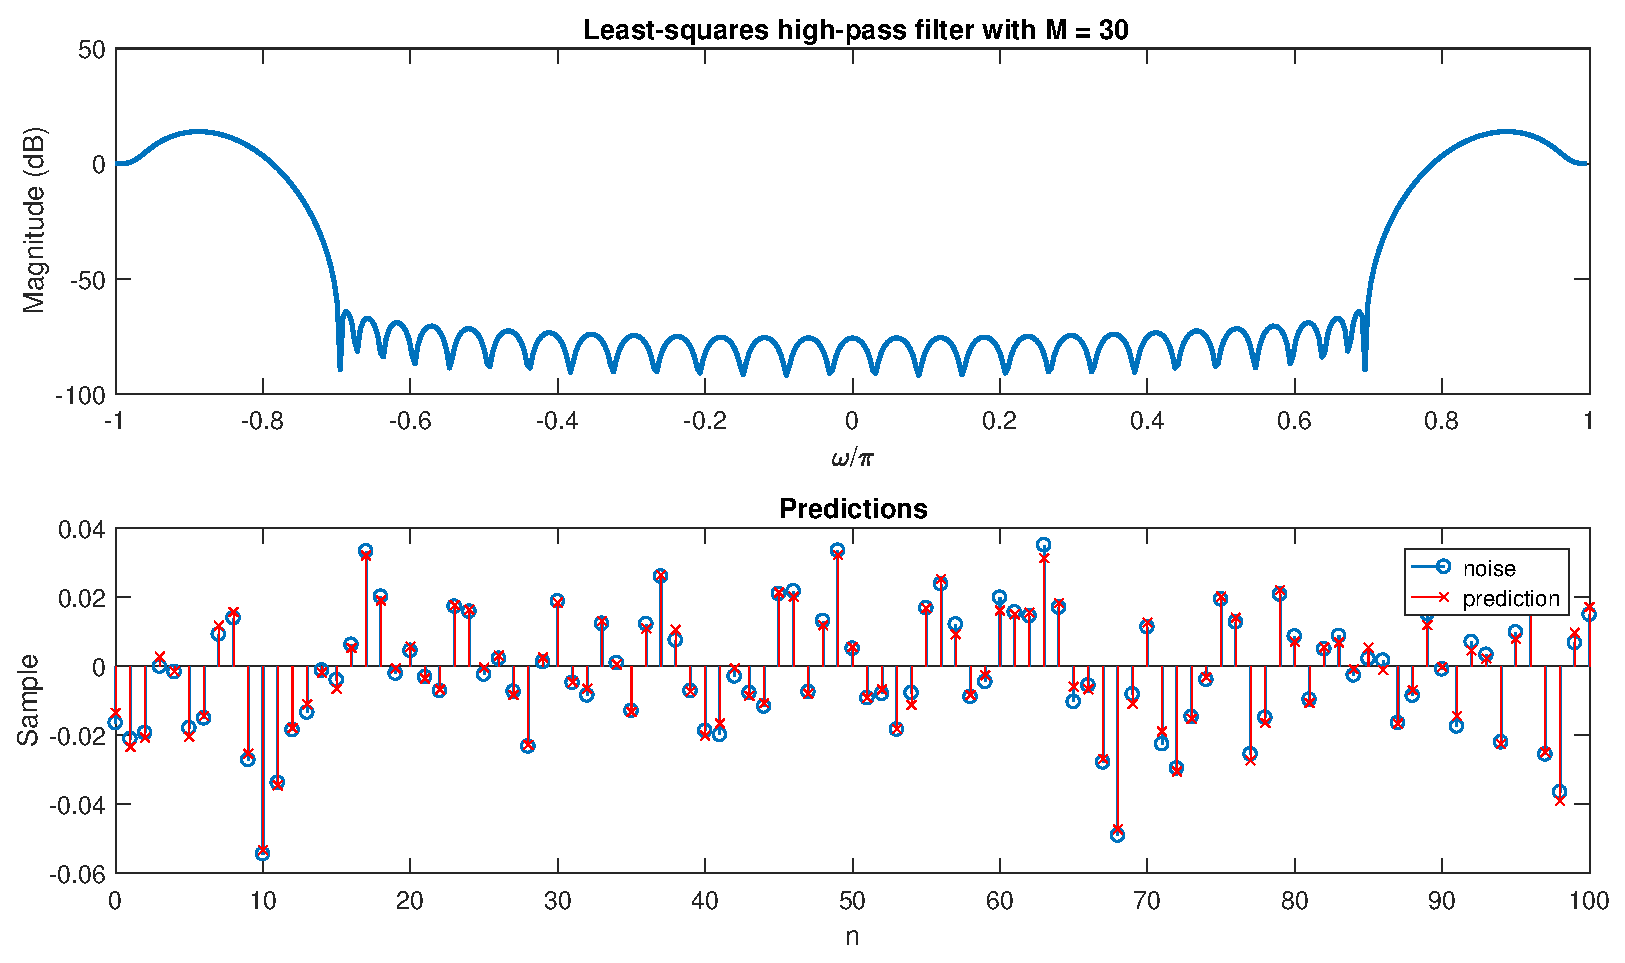
\includegraphics[scale=0.35]{figs/predicting_bandlimited_signals_example.eps}
	\end{center}

	Code available on Canvas: Matlab/predicting\_bandlimited\_signals.m.
\end{frame}

%
\begin{frame}{Summary}
	\textbf{Impulse invariance}
	\begin{itemize}
		\item The impulse response of the continuous-time system is sampled and scaled by $T$. In FIR implementations the impulse response is truncated up to a specified number of samples. In IIR implementations the discrete-time system is obtained analytically.
	\end{itemize}
	
	\textbf{Bilinear transformation}
	\begin{itemize}
		\item The bilinear transformation maps the left-hand side of the $s$-plane into the unit circle in the $z$-plane. This non-linear mapping leads to frequency warping, which can be mitigated by frequency pre-warping. Oversampling also mitigates frequency warping.
	\end{itemize}
	
	\textbf{FIR filter design by windowing}
	\begin{itemize}
		\item Design by windowing is almost an art form
		\item The Kaiser window is a nearly optimal choice
	\end{itemize}

	\textbf{Optimal FIR filter design}
	\begin{itemize}
		\item Optimal FIR filters minimize some characteristic of the weighted error
		\item The Parks-McClellan method minimizes the maximum weighted error
		\item The least-squares method minimizes the mean-square weighted error
	\end{itemize}	
\end{frame}


\end{document}
